\documentclass[fleqn,10pt]{wlscirep}
\usepackage[utf8]{inputenc}
\usepackage[T1]{fontenc}
\usepackage[switch]{lineno} 
\usepackage{multicol}
\usepackage[demo]{graphicx}
\usepackage[square]{natbib}
%\linenumbers
\title{Bioinformatic Investigation of the Zic1/2 binding  reveals novel co-factors in Zic-mediated gene regulation in the cerebellum}

\author[1]{Melyssa Minto}
\author[2]{Emiliano Sotelo}
\author[3]{Vijyendra  Ramesh}
\author[3,*]{Anne E. West}
\affil[1]{Duke University, Computational Biology and Bioinformatics, Durham, 27710}
\affil[2]{Duke University, University Program of Genetics and Genomics, Durham, 27710}
\affil[3]{Duke University, Neurobiology, Durham, 27710}
\affil[*]{corresponding author: west@neuro.duke.edu}

\keywords{Zic, Transcription Factor}



\begin{abstract}
The family of Zic transcription factors (TFs) are required for cerebellar development, and their binding is highly enriched at developmentally regulated enhancers active in cerebellar granule neurons at the progenitor stage around postnatal day 7 (P7) and the mature adult stage at P60 in the mouse cerebellum. Interestingly, Zic1/2 ChIP-seq data reveal that the Zics change their binding profile over time. To characterize these differences in Zic targeting between early and late cerebellar maturation, we compared the sequence underlying Zic Peaks, their relationship with active chromatin and gene expression at P7 and P60. From this we found Zic peaks tend to be large and bind open-active chromatin. Strikingly, Zic peaks shift from binding at promoter proximal regions at P7 to distal enhancer regions at P60.  We hypothesize that other TFs collaborate with the Zic TFs to change their binding targets and affect their regulatory activity. A multi-tiered approach was used to predict TF binding at those Zic ChIP sites. We assessed motif enrichment (HOMER) and in-vivo TF binding profiles (BART) to determine putative TFs collaborating with Zic to drive this regulation. We then validated the presence of the predicted TFs in granule neurons using gene expression. This workflow identified known and novel distinct collaborators of Zic between early and late development. Early collaborates of Zic includes bHLH factors and chromatin remodelers whereas late collaborators of Zic are activity regulated TFs which are markers of synaptic maturation. To identify Zic’s developmental gene targets in cerebellar maturation, we used H3K4me3 PLAC-seq data, which captures promoter-enhancer loops from the adult mouse cerebellum and Hi-C data from the young mouse cerebellum to map genes to Zic bound enhancers. This revealed Zic as a transcriptional activator of late developmental genes in the cerebellum. Using this same approach with in vitro Zic KD, we were able to identify Zic dependent developmental gene targets which have functions in axonogenesis, axon guidance, and ion channel signaling, which are integral in proper maturation of a neuron. These integrated analyses reveal how Zic and other TFs regulate temporal expression of CGN developmental genes and provides information that will enhance our understanding of the molecular mechanisms that regulate the mode of TF function at enhancers.
\end{abstract}

\begin{document}

\flushbottom
\maketitle
\thispagestyle{empty}

\begin{figure*}[ht]
\centering
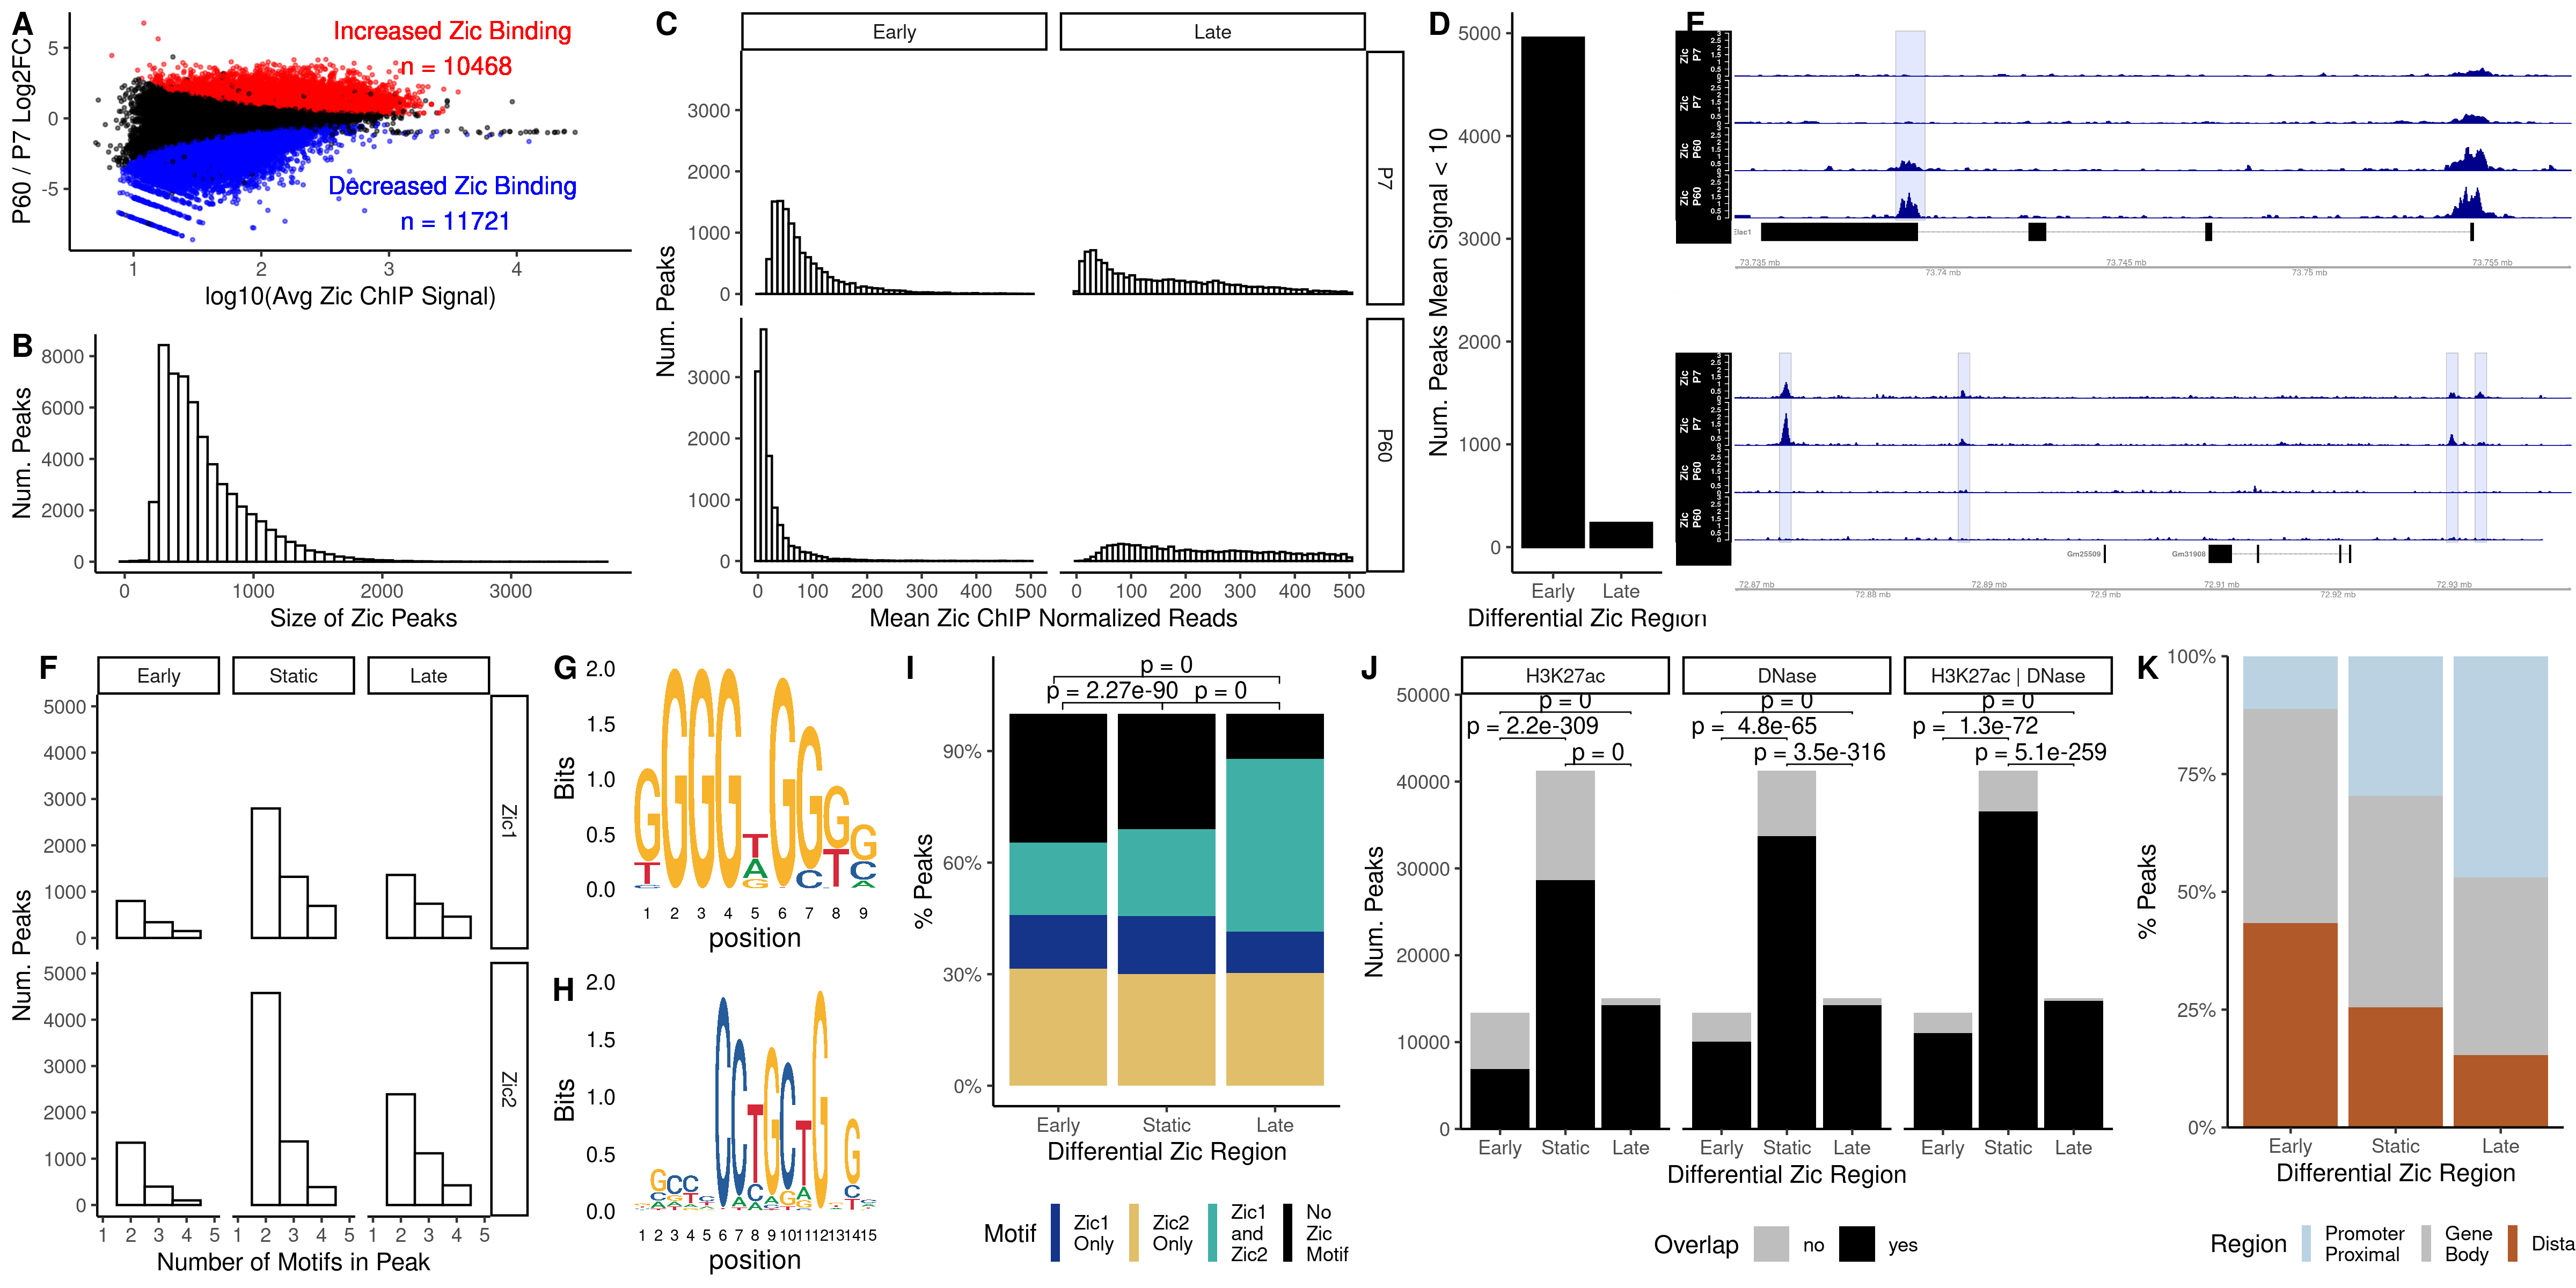
\includegraphics[width=.95\textwidth]{../figures/figure1.png}
\caption{ Zic1/2 Binding is dynamic across cerebellar development. A) MA plot comparing Zic ChIP peaks called by \texttt{macs2} at postnatal day 7 (P7) and postnatal day 60 (P60). B) Distribution of the mean normalized reads in early and late enriched Zic peaks at P7 and P60. C) Total number of  dynamic Zic ChIP peaks that were either completely lost or completely gained over development. D) Example tracks of peaks that were completely gained and completely lost. E) Distribution of the the size(widths) of Zic peaks). Consensus sequence of  F) Zic1 and G) Zic2 motifs found in Zic peaks. H) Distribution of the number of Zic1 and Zic2 motifs in early, static, and late peaks. I) Proportion of Zic1 and Zic2 motifs found in the dynamic and static Zic ChIP peaks. J) Overlap (black) or nonoverlap (gray) of d Zic ChIP peaks with H3K27ac alone, DNase alone, and either DNase or H3727ac. K) The genomic loci of Zic ChIP peaks change from P7 and P60.}
\label{fig:Zicpeaks}
\end{figure*}

\section*{Introduction}
Even though each cell in an organism has the same DNA sequence, cellular differentiation arises from differential gene expression which is achieved through by cis- and trans- regulation of gene expression. Genes are known to be regulated by the DNA’s epigenome. To discover the epigenomic regulation of a specific cell population, computational methods can be used to analyze high throughput sequencing assays for transcription factors (TFs), and histone tail modifications. We can begin to better understand the molecular mechanisms that drive cell type specific differentiation by first finding the TFs involved. Additionally, understanding histone tail modifications, which can be used as proxy for chromatin configuration, will allow us see how chromatin dynamics throughout development lead to the regulation of specific gene expression programs. Although, TF binding is sequence specific; it is also depending on the chromatin landscape and which chromatin is available to be bound. Gene expression, chromatin accessibility, and TF binding can be combined computationally to make whole genome prediction of TF binding and regulation.

TFs are sequence specific DNA binding proteins that regulate the transcription of genes. Inherently, next generation sequencing data can be used to search for transcription factor binding sites (TFBS).  TFs are typically expressed in a precise spatiotemporal pattern when cued to regulate their target genes \cite{}. Aside from sequence binding affinity, there are both intrinsic and extrinsic properties of TFs that make TF binding vary in respect to cell type and cell state.  Intrinsic properties include splice variants, DNA binding domains, whether it can participate in multi-meric binding, post-translational modifications, and/or multiple folding conformations \cite{Siggers2014Protein-DNACodes, Slattery2014AbsenceGenome}. Extrinsic properties include co-factors and their protein recruiting affinity's (cooperative or not), allosteric interactions between other proteins and DNA \cite{Siggers2014Protein-DNACodes}. These properties allow a single TF have the ability to have specific context dependent binding. We can leverage multi-omic data to generate testable hypotheses for context-dependent binding of TFs.
 
To study chromatin dynamics and transcription factor binding over cellular development and maturation, we use the cerebellum as it is strong model system due its homogeneity and prolonged postnatal development.  It is a fairly homogeneous cell population made up of CGNs (85-90\%), interneurons (2\%) Purkinje cells( \textless 1 \%) , Golgi Cells ( \textless 1 \%), and astroglia (5-15\%) \cite{Frank2015RegulationCerebellum}. The cerebellum is an easy to access area of the brain and it has a prolonged postnatal development in mice making it a very tractable system to use\cite{Wang2001GeneticDevelopment}. 

A previous study has shown strong evidence that Zic1/2 works in maturing CGNs regulating developmental genes. Zics are a family of five C2H2 zinc finger TFs that have been thought to derive from the Glioma-associated oncogene factors (Glis) ancestral family \cite{Tohmonda2018IdentificationProteins, Ishiguro2018LinkExpression}. Motifs of the Zics, a family of $C_2H_2$ Zinc Finger TFs, have been previously found in enhancer regions in early and mature stages of CGN development. The expression of Zic1 and Zic2 remain constitutive throughout cerebellar development indicating that Zic1 and Zic2 are playing a role at at the mature time-points. ChIP-seq data reveal that Zic1/2 binding is dynamic between postnatal day 7 (P7) and postnatal day 60 (P60) (Figure \ref{fig:Zicpeaks}A). Furthermore, Zic1/2 KO in cultured granule cells showed mis-regulation of two sets of genes, canonical early developmental genes that failed to be down-regulated and a set of late developmental genes that failed to be up-regulated \cite{Frank2015RegulationCerebellum}. Previous studies have also suggested that Zic2, as well as the rest of the Zic family because of high homology, can act as an activator or repressor depending on the context \cite{Ishiguro2018LinkExpression, Himeda2013Pax3Enhancer, Luo2015Zic2Specification, Hatayama2018RoleRemodeling.}. These data suggest that Zic1/2 are regulating both via activation and repression at the mature time point in cerebellar maturation. These regulatory mechanisms of Zic mediated activation and repression have yet to be described.
 
We hypothesize that there are underlying differences in the sequences Zic1/2 binds to in early and late stages of CGN maturation. In this study we use an integrative bioinformatic workflow to assess multiple characteristics of the sequence of Zic binding in the cerebellum.  This workflow revealed novel co-factors of Zic and mechanisms for Zic dependent gene regulation. We predicted distinct transcription factors that bind near Zic in early and late CGN maturation and validate Zic dependent developmental targets genes.

\begin{figure*}[!ht]
\centering
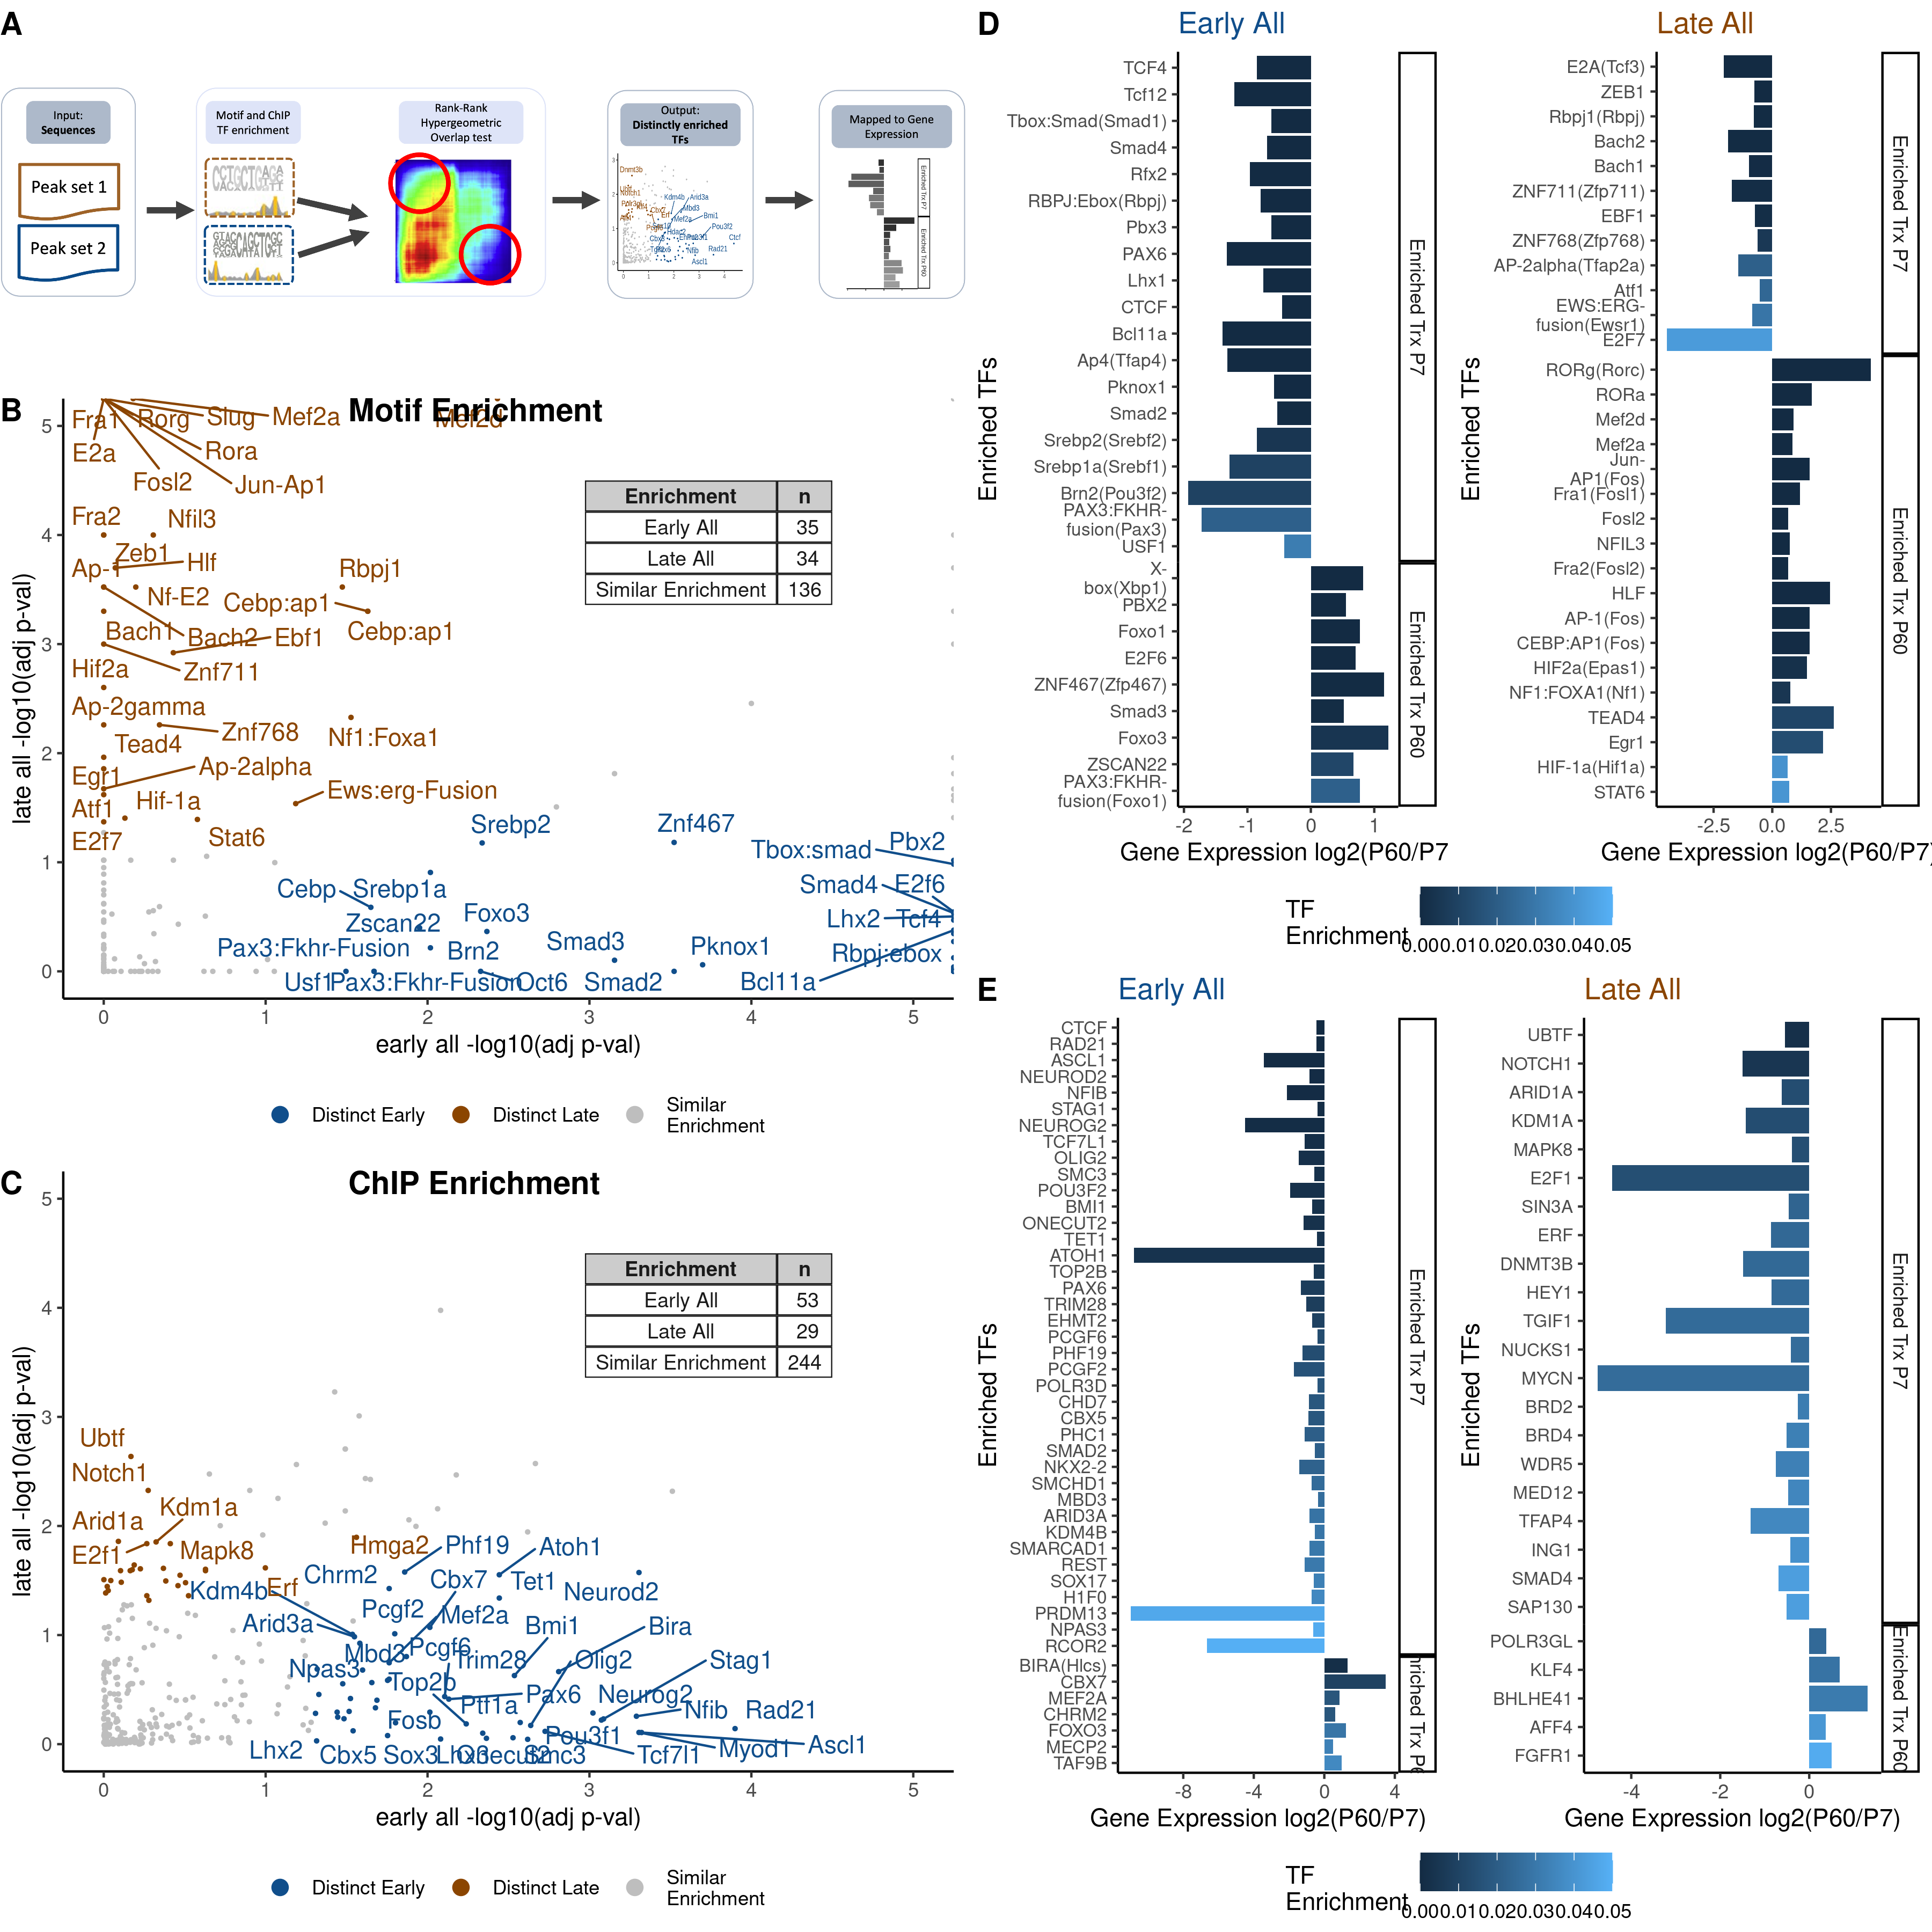
\includegraphics[width=.95\textwidth]{../figures/figure2.png}
\caption{ Distinct TFs are enriched between early and late Zic binding. Motif enrichment analysis using \texttt{Homer} and ChIP overlap enrichment analysis using \texttt{Bart} was performed on early and late Zic binding sites. A ranked hyper-geometric overlap test was performed to identify the distinctly enriched A) motifs and B) ChIP profiles between early and late Zic sites. These TFs C) motifs and D) ChIP profiles in early and late Zic sites were filtered for transcriptional enrichment at the respective time-points. The size of each point is the average expression of the mapped gene at the respective time point. E) The proportion of of ChiP peaks that are co-occupied by Zic peaks colored by the enrichment of the Zic peak (red - enriched at P60, blue - enriched at P7, black - static, and grey - no Zic peak) and F) the proportion of overlap (grey) or nonoverlap (black) of ChIP data sets that overlap Zic peaks separated by P7 enriched, static, and P60 enriched peaks (Right) for Atoh1 at P5 \cite{Klisch2011InDevelopment}. G-H) Example tracks of P5 Atoh1 overlapping with Zic binding throughout development. }
\label{fig:DistinctTFs}
\end{figure*}

\section*{Results}
\subsection*{Zic binding shifts from enhancers to promoters across CGN maturation} 

To characterize the genomic features of Zic binding at early and late stages of CGN maturation we used the data from the 2015 Frank et al. study \cite{Frank2015RegulationCerebellum} and realigned it to the mm10 Gencode genome to interrogate Zics binding and in reference to chromatin activity and gene bodies. We first repeated the differential binding analysis of 56,941 merged Zic ChIP peaks between P7 and P60. This revealed  10,488 peaks enriched at P60 (late), 11,721 peaks enriched at P7 (early), and 34,752 static Zic peaks (Figure\ref{fig:Zicpeaks}A).  Of the dynamic Zic peaks, many were not specific to either time point but instead changed in peak height (i.e. the number of reads mapped to the peak). The distribution of the average reads in each peak shows  that very few late Zic peaks had a low (\<10 normalized ) average reads at P7 or P60, whereas there is a much higher number of early Zic peaks with low average reads ( Figure \ref{fig:Zicpeaks}B). To determine the number of peaks that were time-point specific, we compared the number of dynamic peaks that have an average read \< 10 for one time point  indicating a dramatic loss or gain of peak. Approximately 5000 peaks were specific to P7 and 400 were specific to P60 (Figure \ref{fig:Zicpeaks}C). Overall, early Zic sites tend to be completely lost where as late Zic sites tend to gain in peak height. The loss of Zic is what defines its binding late instead of gaining binding at new sites suggesting that Zic is refining its binding targets over time

The width of Zic ChIP peaks sizes are 528bp on average (Figure \ref{fig:Zicpeaks}E) which could allow for binding of multiple Zic TFs. To further assess the composition of Zic peaks, we looked for the Zic motif sequences in early versus the late peaks and calculated the percentage of Zic ChIP peaks that contained either Zic1 motifs (Figure \ref{fig:Zicpeaks}F) or Zic2 motifs (Figure \ref{fig:Zicpeaks}G) using FIMO.  
Many of these peaks, even though they are large will only have the a few Zic1 and Zic2 motifs ranging from 0 - 4 occurrences each (Figure \ref{fig:Zicpeaks}H). Among the early and static peaks, the Zic2 motif was the most commonly found, with a smaller proportion of peaks containing the Zic1 motif with or without Zic2. Greater than 25\% of peaks contained neither motif, suggesting that Zic might bind these sites in a non-canonical way either through targeting different sequences or via indirect binding. By contrast the late sites were more highly enriched for peaks with both Zic1 and Zic2 (Figure \ref{fig:Zicpeaks}H,I). This supports Zic binding is consolidating at the late time-point with the increase in both motifs and greater Zic binding intensity.

We hypothesized that Zics are binding to candidate regulatory elements (CREs). To assess the difference between early and late Zic binding to CREs, we examined the overlap of Zic peaks with DNAse hypersensitivity (DHS) and the acetylation of the lysine residue at N-terminal position 27 of the histone H3 protein (H3K27ac) as markers of CREs. Early, late, and static Zic binding sites were all largely within regions of active chromatin indicated by overlap with DHS sites or H3K27ac (Figure \ref{fig:Zicpeaks}J). Specifically, this demonstrates that Zic is primarily binding to open and active chromatin and at an increasing rate throughout development. 

Genome-wide binding profile studies have revealed that transcription factors differ in their sites of action in the genome. Some TFs (such as SP1) bind preferentially at proximal promoter regions, whereas others (such as Npas4 for example) are more likely to be found bound at distal enhancer regions \cite{Kaczynski2003Sp1-Factors, Lyons2011MechanismsTranscription}. We aligned the early, static, and late Zic ChIP peaks to gene positions in the genome and were surprised to see that the distribution of Zic significantly shifts across CGN maturation. Whereas the early Zic peaks are about evenly split between gene bodies and distal enhancers, with fewer sites in proximal promoter, the late sites shifted in distribution substantially from distal to proximal sites. The static sites showed and intermediate distribution that was largely equal across the three compartments (Figure \ref{fig:Zicpeaks}K). All these data suggests that Zic is consolidating on a common set of CREs in late sites. 

\subsection*{Distinct TF binding sites are enriched in early and late Zic ChIP peaks}

We next asked what is causing differential targeting of Zic binding between P7 and P60. We considered Zic might bind together with other co-factors that show differential expression or genome recruitment between these stages of CGN maturation. Specifically, we hypothesized that TFs working with Zic early versus late would 1) bind close to Zic and this be within the regions defined as Zic ChIP peaks and 2) would be differentially expressed during development. We used a  multi-pronged approach to identify these high probability Zic co-factor TFs. First we searched the genomic locations of the early and late Zic ChIP peaks for TFs that were shown in previous ChIP studies to be enriched at these genomic loci using BART \cite{Zhenjiawang2018BART:Profiles, Ma2021BARTweb:Analysis}. In parallel, we interrogated the sequence of the Zic ChIP peaks for TF motifs using Homer \cite{}. The combination of these methods allows us to consider both indirect genomic association with Zic as possible methods for co-regulation of these regions with Zic and direct DNA binding by looking at the sequences. 

The tools Bart and Homer each interrogate a large set of overlapping TFs (Figure \ref{fig:HomerBart}A). When we initially looked  independently at TF enrichment in early and late Zic peaks we found that many enriched TFs were shared in the early and late sites (Figure \ref{fig:HomerBart}B-C).  To identify statistical differences of putative TFs between early and late peaks in the Bart and Homer analysis, we used a Rank-Rank Hyper-geometric  overlap test to find TFs that are the distinctly enriched between peaks from the two time points (Figure \ref{fig:HomerBart}D-E). Finally, each predicted TF whose motifs or ChIP profiles were enriched, for being developmentally expressed(Figure \ref{fig:DistinctTFs}). This workflow revealed distinct sets of TFs predict to be regulators of Zic binding in early and late stages of CGN maturation(Figure \ref{fig:DistinctTFs}A-B). Enriched TFs were filtered for concordant temporal transcriptional enrichment. Out of 205 enriched motifs, 35 are distinctly enriched in the early Zic peaks, and 34 and distinctly enriched in the late Zic peaks set (Figure \ref{fig:DistinctTFs} A-B). Out of the 326 TF whose ChIP binding were enriched in the early and late peak sets, 53 were distinctly enriched early, and 29 were distinctly enriched late (Figure \ref{fig:DistinctTFs}A-B).  

\subsection*{Workflow captures previously identified TFs known to work with Zic in early neurogenesis and chromatin remodelers}
TFs that were distinctly enriched in early Zic sites as well as transcriptionally enriched early included factors involved in cell proliferation via Wnt, Fgf, Notch and Smad signaling (Figure \ref{fig:DistinctTFs}). These factors include Tfap4 which is upstream  of Wnt signaling \cite{Medina-Martinez2020TheDevelopment, Song2018TranscriptionCarcinoma}, RFX proteins which are upstream of FGF activation \cite{Hsu2012CiliogenicPromoter}, TCF proteins \cite{Shy2013RegulationSignaling} which are a co-effectors in  Wnt/$\beta$-catenine pathways and downstream targets of these pathways including  Atoh1, Ascl1, Sox17, and Neurog2 \cite{Dennis2019BHLHReprogramming, Zhu2019pBCL11ACancer/p, Lacomme2012NEUROG2Cycle, Katoh2018MultilayeredReview, Lebensohn2016ComparativeSignaling}. Smad proteins were also enriched in the early Zic sites which are downstream activators of Tgf-beta signaling and downstream of BMP signaling \cite{Liu2021SMAD4Pathways, Nickel2019SpecificationSignaling,Derynck2003Smad-dependentSignalling}. Consistent with the evidence that the Zic TFs play important roles in early differentiation of CGNs, early Zic sites are also enriched for factors that are important in axon guidance (Nkx2.2) \cite{}, and cellular migration (Pbx3,Pknox1, Lhx1) \cite{}. Overall, Zic peaks at P7 were enriched for Homeobox and bHLH factors TF (Figure \ref{}). This is consistent with previous studies implicating Zic as a regulator of pro-neural bHLH factors in early proliferative stages neuronal differentiation \cite{Aruga2018ZicDisease}.

Most notably, the TF is Atoh1 is greatly transcriptionally enriched at P7. In the Cerebellum, the bHLH factor, Atoh1 has been shown to be expressed in the rhombic lip progenitor zone to regulate the expression of other TFs such as Pax6 and give rise to cerebellar granule neurons between the stages of E12.5 - P14 \cite{Aruga2018ZicDisease, Yeung2014WlsDevelopment, Wang2005Math1Cerebellum, Ben-Arie1997Math1Neurons}.To validate the predicted co-factors of Zic in early and late CGN development, we examined the overlap of binding profiles of available ChIP-seq data in the developing mouse cerebellum. The overlap of CGN fate-determining TF Atoh1 with early, static, and late Zic ChIP-seq peaks was calculated. Comparing P5 cerebellar Atoh1 ChIP peaks to developmentally regulated Zic peaks reveal that ~55\%  Atoh1  peaks do in fact overlap with Zic peaks (Figure \ref{fig:DistinctTFs}E-H). Atoh1 ChIP overlaps at early Zic peaks at a greater percentage than static and late Zic peak (p-value < 0.05) (Figure \ref{fig:DistinctTFs}E-F). These results validate that this workflow that integrates gene expression and sequence underlying ChIP peaks to predict functionally relevant TFs that are enriched in this developmental context.

A strong signature of chromatin remodeling factors whose ChIP binding profiles and motif were enriched in the early Zic binding sites. TFs that are members or interact with of cohesin complex  (CTCF, Rad21, Smchd1, Smc3, Stag1, and Top2b), Polycomb  complexes (BMI1, Pcgf2, Pcgf6, Phc1, Phf19, and Usf1 ), HP1 complex (Cbx5, Trim28), Nurd Complex ( Chd7, Mbd3, Trim28 ), REST (Rcor2, Rest) complex and BAF complex (Arid3a, Bcl11a, Smarcad1, Top2b) are distinctly enriched in early Zic binding (Figure\ref{fig:DistinctTFs}A,C). In addition to members of these large complexes, factors involved in demethylation including Tet1, Kdm4b, and methylation Ehmt2, and Prdm13 are enriched in early sites. The linker protein H1.0 (H1f0) that is associated with proliferation and differentiation is also an enriched in early Zic binding \cite{DiLiegro2018H1.0Differentiation}. Unlike the pro-neural and signaling TFs enriched discussed earlier, this suggest a novel mode of Zic mediated gene regulation in interacting with chromatin remodelers to push forward CGN maturation.

\subsection*{Differentiation and Synaptic maturation markers are late collaborators of Zic}

Unlike the study of Zic in progenitors, very little is known about the functions of Zic in mature neurons, thus we had little premise for what to expect in the analysis of co-factors in the late Zic binding sites.  Here we show that RORa and RORc, two factors involved in retenoid acid signaling promoting differentiation, are distinctly enriched at late Zic sites (Figure\ref{fig:DistinctTFs}C). Other enriched TFs that are markers of differentiation include, Klf4 and Hif1a\cite{}(Figure\ref{fig:DistinctTFs}D). 

Most strikingly, the Homer results suggest a key role for activity-dependent transcription in the co-regulation of Zic. On a genomic level, activity regulated genes are important in regulating this refinement. In the late Zic sites, we see enrichment for canonical activity regulated TFs are enriched  including Fosl2, Fos, Jun, Egr1, Mef2a, and Mef2d (Figure \ref{fig:DistinctTFs}C). The AP1 transcription factors have been shown to be capable of promoting accessibility, which could be at play here.  Taken together, late Zic binding is near factors that regulate differentiation and synaptic maturation at P60. 



\subsection*{Mapping peaks to Genes via chromatin loops to determine transcriptional regulation by Zic}

\begin{figure*}[!ht]
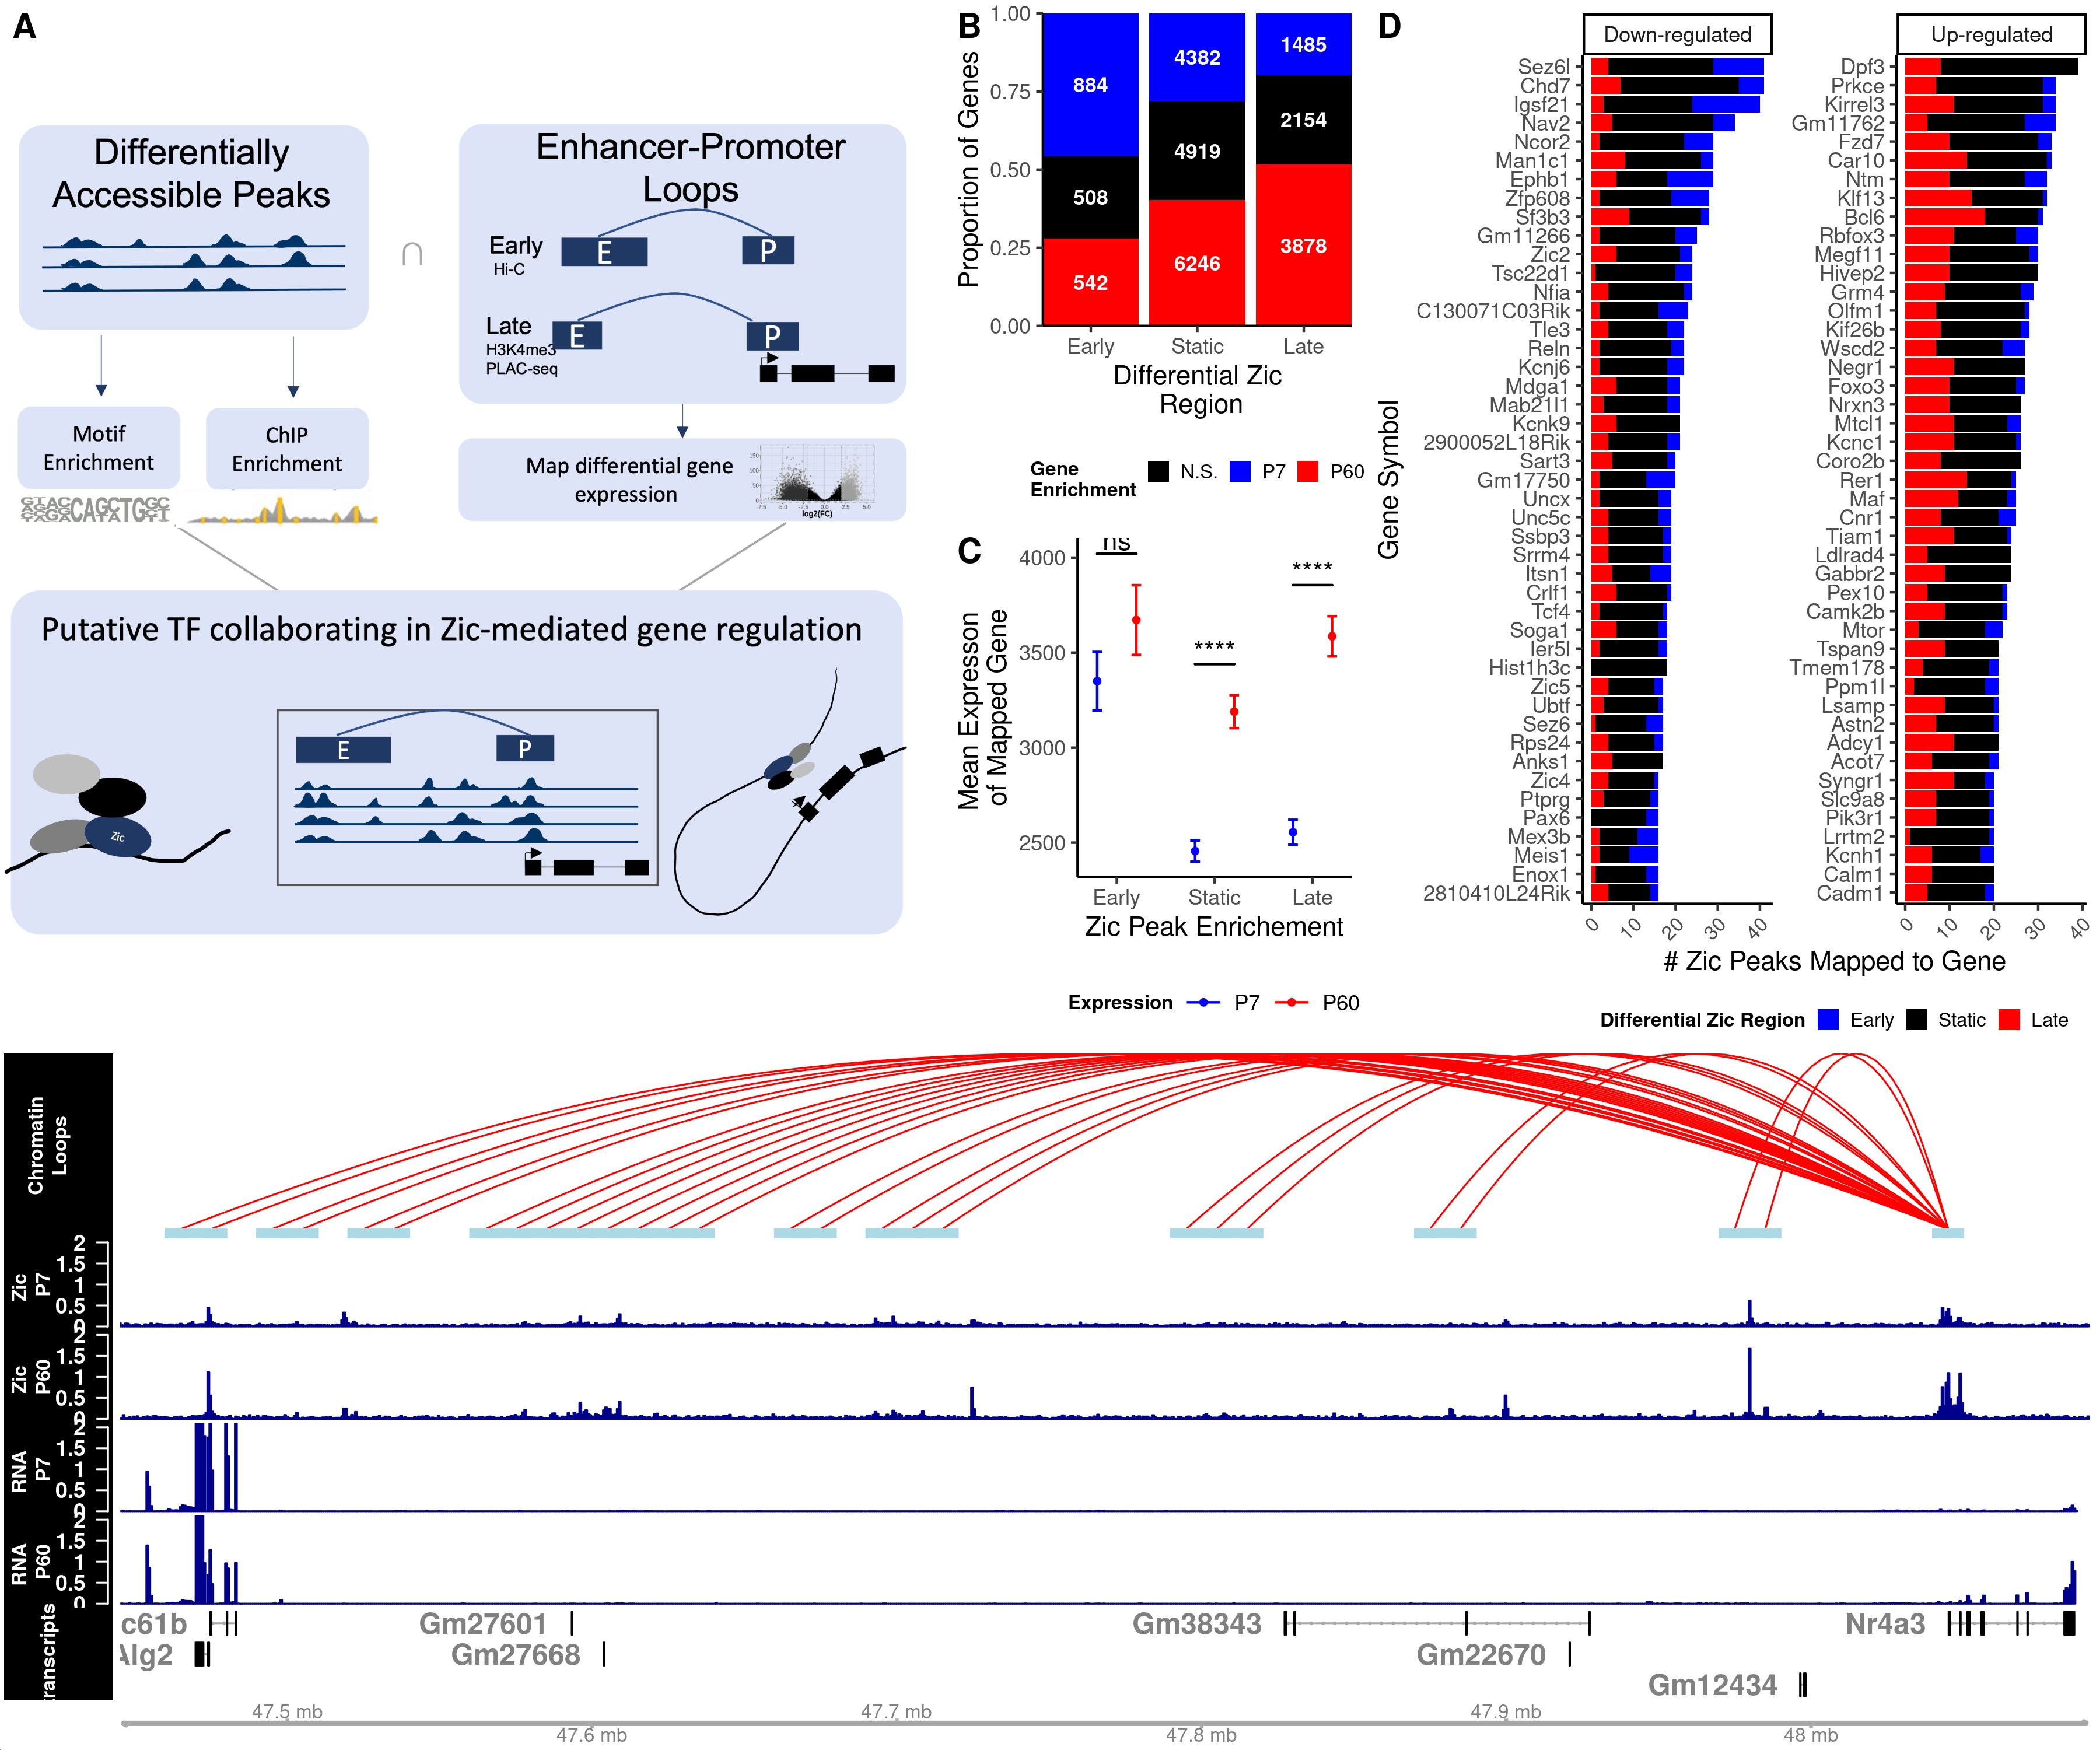
\includegraphics[width=.95\textwidth]{../figures/figure3.png}
\caption{Zic peaks were mapped to genes via chromatin loops derived from cerebellar Hi-C (Goodman et. al. 2020)\cite{Goodman2020TheBrain} and H3K4me3 PLAC-seq (Yamada et al. 2019)\cite{Yamada2019SensoryLearning} data. A) Schematic of peak mapping using chromatin looping data. B) Overall number of genes mapped to Zic peaks that are enriched at P7, P60, and statically bound, C) mean expression of genes at P7 and P60 mapped to P7 and P60 enriched Zic peaks and D) top 50 number of Zic peaks mapped to genes that are differentially expressed between P7 and P60, where red indicates enriched at P60, blue indicates enriched at P7, and black indicates static/constitutive. E) Example tracks of H3k4me3 loops, Zic, DHS, H3k27ac, and Gene expression at P7 and P60.}
\label{fig:peakMapping}
\end{figure*}

Up to this point we have analyzed features of Zic binding with respect to their local sequence and chromatin features, but we have not yet considered the role of Zic binding with respect to transcriptional regulation of genes. As we show in Figure \ref{fig:Zicpeaks}K, at most \textless 50\% of Zic ChIP peaks are in proximal promoters, where they can be expected to regulate the nearest gene. TFs bound far away in linear space from the target genes are thought to come into close three-dimensional proximity with their target gene promoters via structural looping. Thus, to identify the likely target genes of the Zics, and to discover the relationship between developmentally-regulated Zic binding and differential gene expression, we integrated our Zic ChIP data with two different datasets of chromatin conformation \cite{Yamada2019SensoryLearning,Goodman2019RegulationRemodeling} from the developing mouse cerebellum. These published studies that mapped enhancer-promoter loops  had been captured from P4 or P56 cerebellum. One used antibodies against H3K4me3 to perform promoter-centered PLAC-seq from adult mouse cerebellum \cite{Yamada2019SensoryLearning} and the other used Hi-C to identify chromatin loops in cerebellum from young mice \cite{Goodman2019RegulationRemodeling}. We filtered early, late, and static Zic peaks for those that were within anchors of the captured chromatin loops in either dataset (Figure \ref{fig:peakMapping}A, \ref{fig:MappingStats}). 

Though the two methods for chromatin architecture capture used at P4 and P56 differed, we still expected that early Zic sites would preferentially overlap the anchors from P4 and the late Zic sites would preferentially overlap the anchors from P56. Indeed, a higher proportion of anchors from the early anchor dataset mapped to early Zic peaks and vice versa (Figure \ref{fig:peakMapping}B). These data show that we can use chromatin conformation data to predict developmental associations of distal Zic binding sites with genes. 

To determine the relationship between Zic binding and gene transcription we first assessed the average expression level at P7 and P60 of genes that map to early, static, or late Zic peaks. Overall, the expression of all the genes mapped to Zic-containing anchors rose at P60, with genes mapped to the static and late peaks showing significant increases (Figure \ref{fig:peakMapping}C). This suggests Zic has a gene activating role especially in late stages of cerebellar maturation.  

We next asked if the number of Zic binding events was a proxy for regulatory activity by asking if expression at any given time point or fold change in expression from P7 to P60 was a function of the number of Zic peaks that mapped to a gene. We calculated the number of early, static, and late Zic peaks that could be mapped to each gene (Figure \ref{fig:peakMapping}D). We found no correlation between the number of Zic peaks and distribution of the mapped gene log fold change, average expression, or degree of fold change (Figure \ref{fig:npeakstoGenes}). When we looked at the top 30 genes with most mapped Zic peaks, we saw qualitative evidence that down-regulated genes were more likely to have Zic sites that were eliminated by P60 and that up-regulated genes were most likely to gain Zic sites (Figure \ref{fig:peakMapping}D). However, there was no strict correlation. Thus, Zic binding does not have an linear effect on gene expression.

Finally we considered the possibility that different binding partners might explain the relationship between Zic binding and target gene transcription. We repeated the TF enrichment analysis as performed in Figure \ref{fig:DistinctTFs} but considering only Zic peaks in anchors. We saw that the motifs enriched in all peaks versus looped peaks were highly concordant in the early and late sets (Figure \ref{fig:loopved_all}). Subsequently, the results of distinct TFs between the looped early and looped late Zic peaks were also very similar to ones shown in Figure \ref{fig:DistinctTFs} (Figure \ref{fig:DistinctTFs_looped}). Taken together, we conclude that the characteristics of all Zic peaks and looped Zic peaks are highly homologous.

\subsection*{Identification of genes that require Zic1/2 for their developmental expression}
\begin{figure*}[!ht]
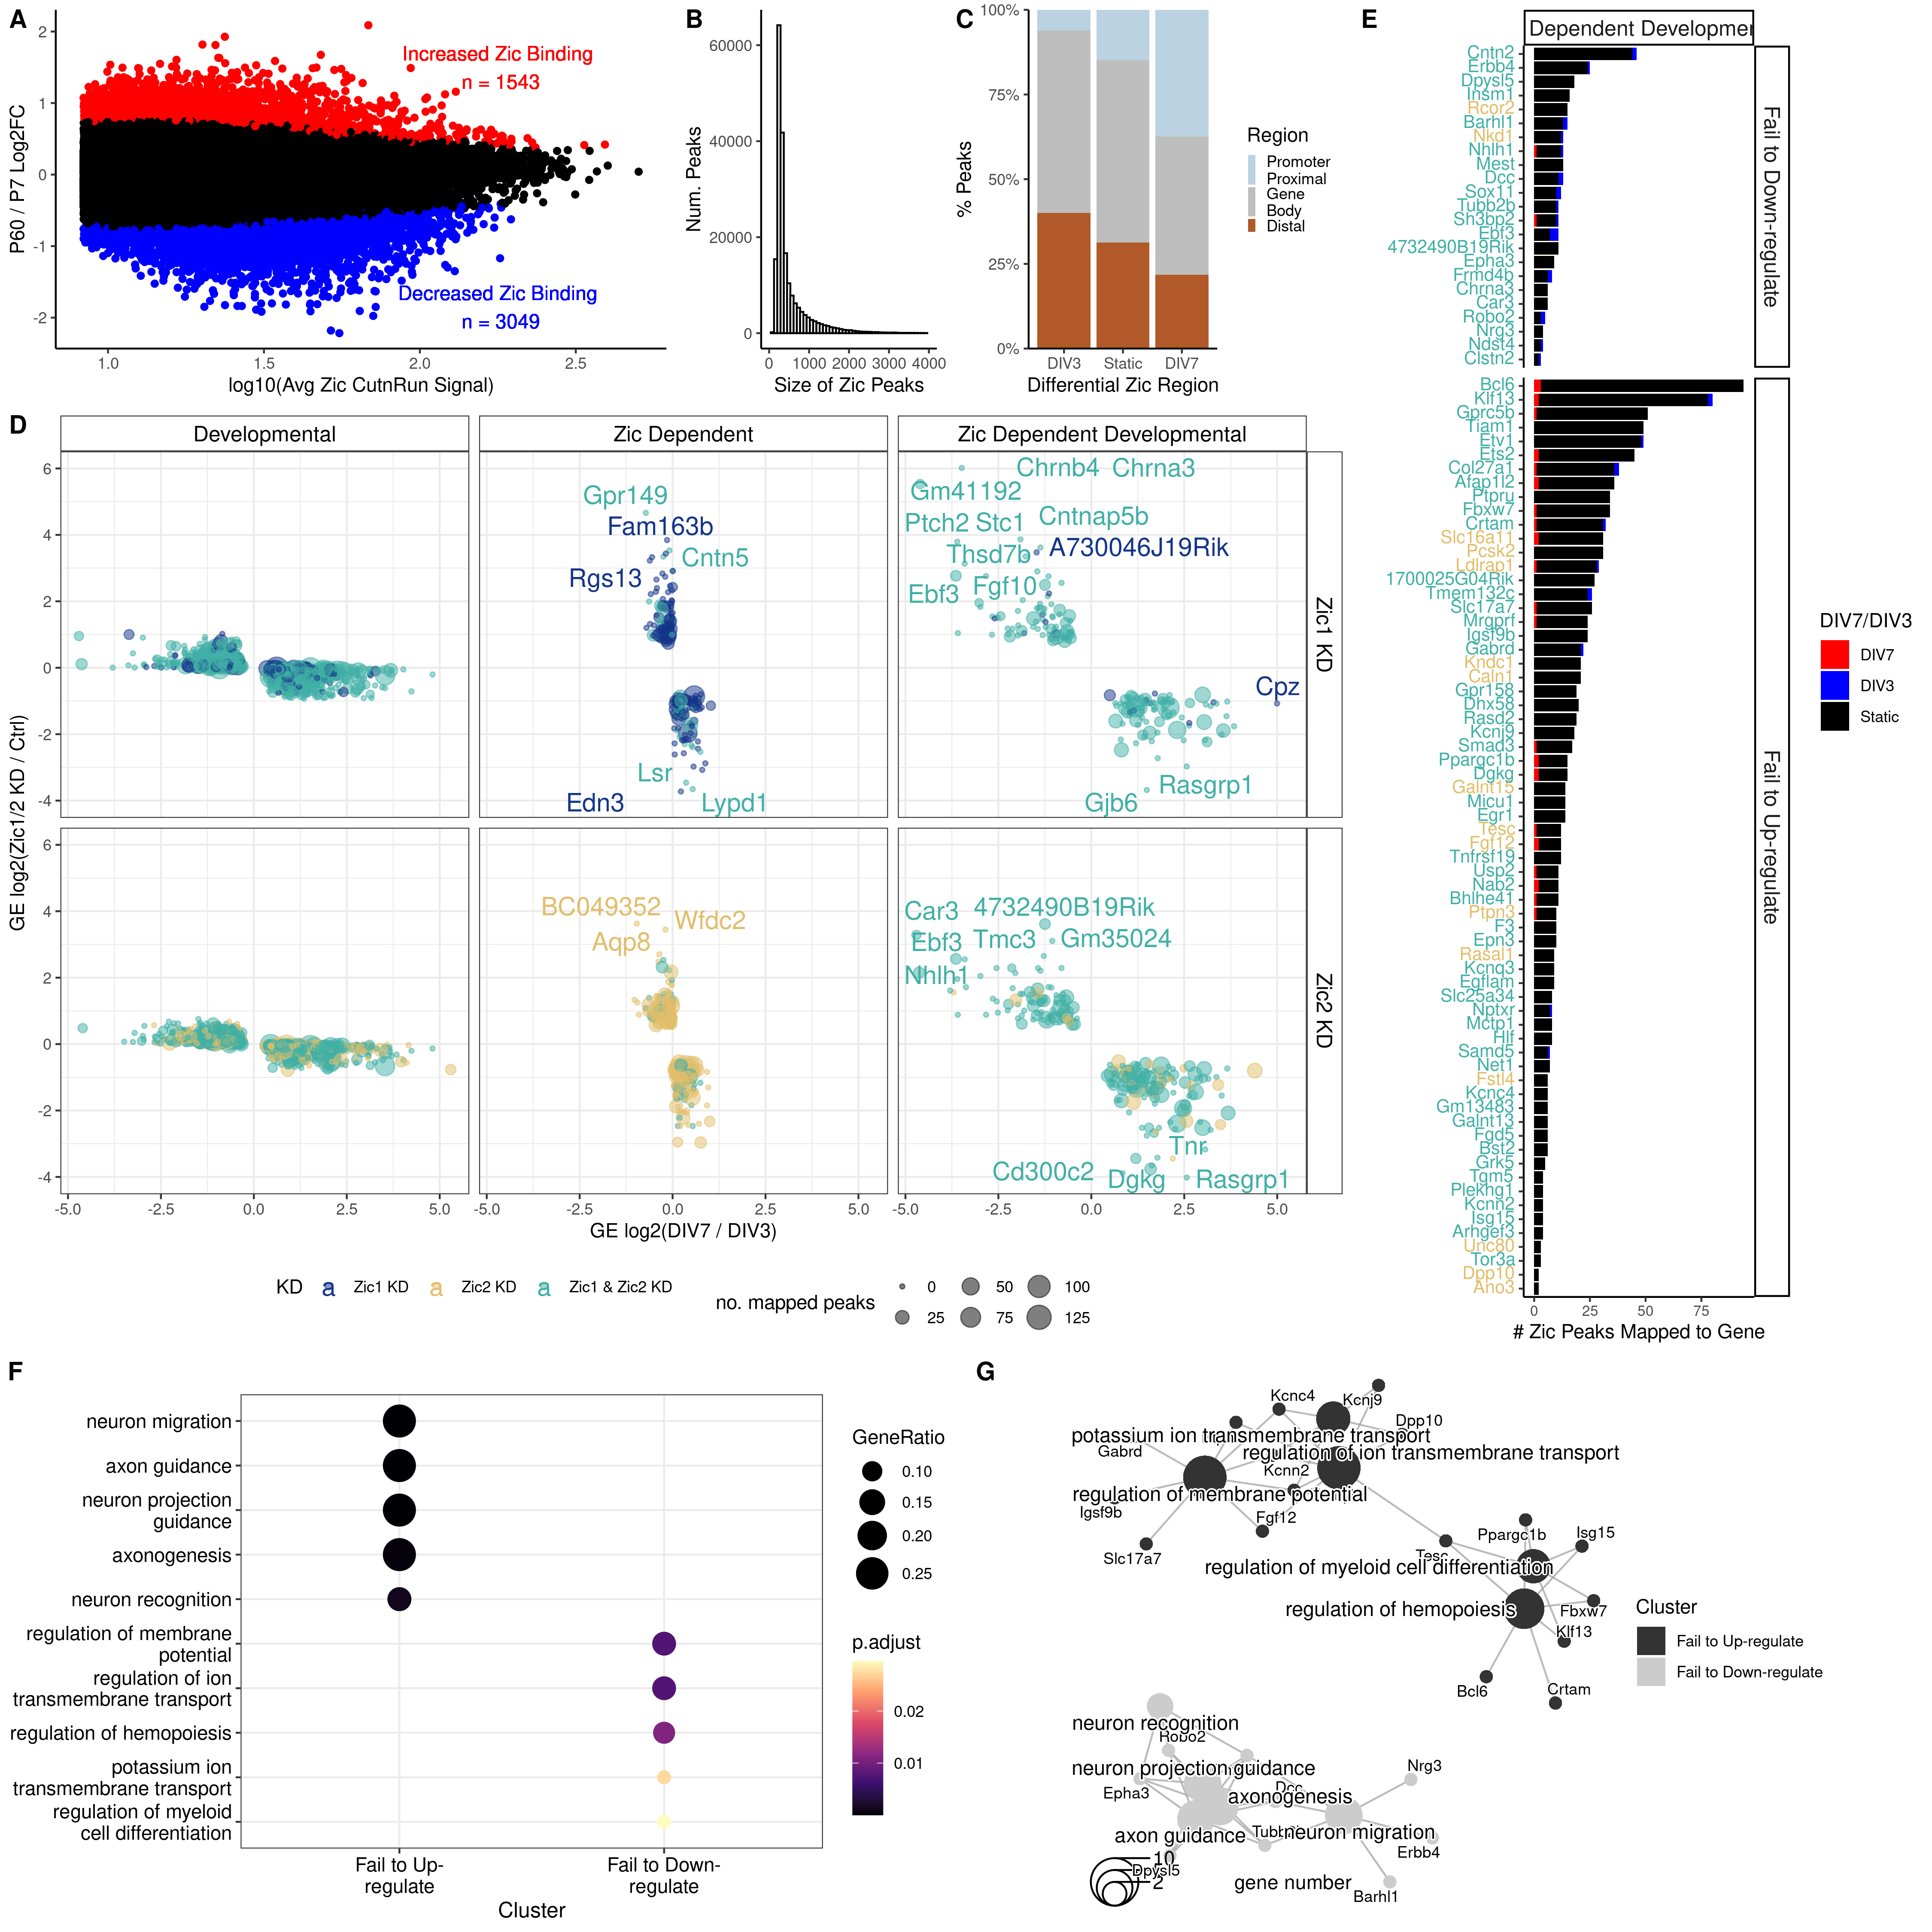
\includegraphics[width=.95\textwidth]{../figures/figure4.png}
\caption{Direct Zic targets were estimated using Zic1 or Zic2 KD. A) Fold-Changes of discordantly regulated genes between DIV7/DIV3 and Zic1/2 KD v WT at DIV7 categorized by developmental, Zic dependent and Zic dependent developmental where the colors represent where the gene was mis-regulated by Zic1 KD, Zic2 KD or both and the size of the point represents the number of Zic peaks mapped to the gene. B) MA plot of Zic CUT\&RUN peaks called by \texttt{seacr} at3 days in-vitro (DIV3) and 7 days in-vitro (DIV7). C) Distribution of the the size (widths) of Zic peaks. D) The genomic loci of Zic CUT\&RUN peaks in DIV3 enriched, Static, ad DIV7 enriched peaks.  E) Number of Zic CUT\&RUN peaks at DIV3 and DIV7 were mapped to each Zic dependent developmental genes. F) Significant GO categories for the sets of genes that require Zic for developmental up- or down-regulation and G) clustered. }
\label{fig:ZicKD}
\end{figure*}

In our prior study we found that knockdown of Zic1 or Zic2 in CGNs taken from P7 brain and differentiated in culture leads to both increases and decreases in gene expression. However, we were unable at the time to resolve whether the genes that changed expression upon loss of Zic were direct transcriptional targets of Zic or whether they were changed indirectly as a result of Zic knockdown. Here to identify the direct targets of Zic TF regulation in cultured CGNs, we conducted CUT\&RUN-seq with our Zic1/2 antibody to map Zic binding sites across the genome after 3 or 7 days in-vitro (DIV). We chose these times because they are the same timepoints we used in our previous study to capture changes in gene expression that correspond with differentiation of the CGNs.

To capture the largest overlapping sets of developmentally-regulated Zic1/2-dependent genes, we performed RRHO analyses comparing the differential genes in normal CGN development versus when the Zics were knocked down  (Figure \ref{fig:vitro}D-F). We first reanalyzed the in vitro RNA-seq data sets from Frank et. al. \cite{Frank2015RegulationCerebellum} with updated references and tools by re-aligning them to mm10 Gencode genome and performing differential expression analysis with DESeq2 1.36.0. This resulted in 1388 up-regulated genes, 855 down regulated genes between DIV7 v. DIV3. The same methods were used to re-analyze Zic1KD v. control at DIV7 resulting in 541 differentially expressed genes (up-regulated = 277, down-regulated = 264) and Zic2KD v. control at DIV7 resulting in 738 differentially expressed genes (up-regulated = 303, down-regulated = 435) (Figure \ref{fig:vitro} A-C). We then compared each of the bilateral comparisons against one another to get the sets of genes that were differentially regulated between DIV3 v. DIV7 and Zic1/2 KD v. control which fell into three categories 1) Developmental (n=1582) 2) Zic Dependent (n=455) and 3) Zic Dependent Developmental (n=329) (Figure \ref{fig:ZicKD}A). Of these categories, developmental genes were unchanged by the KD of either Zic1 or Zic2 thus these genes were not dependent on the Zics. The Zic Dependent genes  were affected in either the Zic1 or Zic2 KD but were not developmentally regulated. There are not many Zic Dependent genes that are implicated in both the Zic1 and Zic2 KD revealing some variability in the Zic1 and Zic2 targets. Lastly, the Zic Dependent Developmental (ZDD)  genes were affected by the Zic1 or Zic2 KD and were developmentally regulated suggesting that they either direct or downstream targets of Zic in CGN maturation. 

The ZDD group of genes offered us the strongest opportunity to assess how Zic binding relates to changes in gene expression. To determine the direct Zic targets from the ZDD gene list, we next asked which of these gene had Zic binding at their promoters or enhancers. Differential binding analysis of 49,296 merged Zic CUT\&RUN peaks between DIV3 and DIV7 revealed  1543 peaks enriched at DIV7, 3,049 peaks enriched at DIV3, and 44,704 static Zic peaks (Figure\ref{fig:ZicKD}B). Similar to the in-vivo Zic ChIP peaks, the peak sizes are large enough to allow for binding of multiple TFs with the median size being 317bp (Figure \ref{fig:ZicKD}C). Additionally, the Zic CUT\&RUN peaks show a similar shift from binding distal enhancers to promoter proximal regions as the CGNs mature (Figure \ref{fig:ZicKD}D). Even though Zic is not as dynamic in this culture system as shown in-vivo, they are still represent the in-vivo system well. 

The in-vitro Zic peaks were mapped to genes via chromatin loops in order to determine direct targets of Zic binding. 37 ZDD genes had in-vitro Zic peaks mapped to them and thus were classified as direct Zic targets in CGN development. Peaks mapped to these genes were mostly statically bound (Figure \ref{fig:ZicKD}E). This set of direct targets were then separated in to genes that either failed to up-regulate or fail to down-regulate when the Zics were knocked down. To further understand the functions of Zic targets, GO enrichment analysis was performed on the Biological Processes (BP) terms for these genes (Figure \ref{fig:ZicKD}F-G). Zic targets that failed to be down-regulated were enriched for GO BP terms including "regulation of ion transport channels" and "regulation of membrane potential". Zic targets that failed to be up-regulated were enriched for GO BP  terms including "neuron migration" and "axonogenisis", both of which are important processes in mid to late CGN maturation. Overall these genes showed signatures for neuronal markers that are important in development and synaptic refinement. 

\section*{Discussion}
We sought out to determine the modes of Zic binding in the developing cerebellum by interrogating the sequence that underlies Zic peaks in early and late maturation. We implemented an integrative approach to enhance our understanding of Zic1/2 regulation on a molecular level. Although there were no differences between Zic peaks mapped to gene activation and Zic peaks mapped to gene repression, there was a clear difference between early and late Zic binding. While early Zic sites showed signatures of repressive chromatin remodeling complexes, the late Zic sites showed a novel set of activity regulated genes that are important in late neuronal maturation and synaptic refinement. 
%Some TFs can act as pioneer factors which bind to closed DNA through partial motif match ting to initiate the opening of chromatin, increase activity, and activate programs of gene expression. These Pioneer factors are particularly important in cell fate determination and development\cite{Zaret2020PioneerChanges}.  (move to discussion)

% discussion (Fig1J: data is variable at early stages because of the homogenous cell populations 

%Even though there is great overlap in the database of TFs tested for enrichment in both the BART and HOMER databases (Figure \ref{fig:HomerBart}A), many of the predicted TFs with enriched motifs are not enriched by ChIP profiles (Figure \ref{fig:HomerBart}B-C).

Many studies have implicated Zic in the maintenance of neuronal cell proliferation \cite{ Lim2007Zic3Cells, Janesick2013ERFNeurogenesis, Aruga2002Zic1Differentiation, Ebert2003Zic1Autoregulation }. For example, Zic1 represses differentiation factors in order to increase cell number \cite{Aruga2002Zic1Differentiation}. Some of the predicted TFs enriched in early Zic sites have been described up and downstream of the Zics in several pathways in embryonic development. TCF proteins have been demonstrated to bind with Zic2 to repress  Wnt/$\beta$-catenin signaling \cite{Aruga2018Zic1, Lowenstein2021Olig3Development}. FGF and Notch signaling have been proposed to work concurrently to lead to neurogenesis \cite{Voelkel2014FGFHierarchy} whereas Wnt signaling plays a context dependent role in neurogenesis \cite{Lassiter2014SignalingDelamination}. Zic1/2/3 is known to block Wnt-$\beta$-catenin signaling binding directly to TCF proteins of the $\beta$-catenin complex \cite{Ge2020Zic1Transition, Fujimi2012XenopusPathway, Murgan2015AtypicalPrecursors, Pourebrahim2011TranscriptionSignaling, Aruga2018ZicDisease,Aruga2018Zic1,Lowenstein2021Olig3Development}.  

%Bcl11a have implicated in cerebellar malformations such as holoprosencephaly human and mouse \cite{Aruga2018ZicDisease, Shimbo2017HaploinsufficiencySyndrome}.

% While some of this may be attributed to the different sets of TFs used in the Homer and Bart tools (Figure \ref{fig:HomerBart}A), it still suggests that there are many TFs that are indirectly bound at these Zic sites. 

This workflow identifies novel interactions with Zic and chromatin repressive complexes in the CGN development. Members of Cohesin are enriched at the early Zic sites including CTCF, Rad21, and Smc3. Studies have shown that the 3D architecture of the genome is dynamic between early development and cell fate commitment. While TAD boundaries are relatively stable, local chromatin can undergo massive reorganization as cells respond to signaling or developmental cues which is correlated with changes in gene expression\cite{Zheng2019TheDifferentiation, Bonev2016OrganizationGenome}. For instance, the polycomb complex is linked with maintaining the repression of pluripotency genes \cite{Riising2014GeneWide}. BMI1 and Pcgf2 the major ring  and core components of PRC1 whose role is to maintain repression of genes \cite{Aranda2015RegulationProteins}. Interestingly, Phc1 whose binding is enriched in early Zic sites, has recently been shown to activate  Nanog in a PRC1-independent manner and repress developmental genes in a PRC1-dependent manner \cite{Chen2021Phc1Locus}. These data suggest that Zic interacts with chromatin remodeling factors to regulate gene expression programs important to the developing cerebellum. 

Collaborators of the BAF complex to drive and maintain proliferation were found enriched at early Zic sites. Top2b, a collaborator of BAF to recruit pluripotency pioneer factors including Oct4 and Nanog, was enriched at early Zic sites. Similarly,  Smarcad1, a subunit of BAF that has been shown to be involved in Histone H3/4 turnover \cite{Markert2021Smarcad1Activity}, was  enriched at early Zic sites. BAFs have a varying roles in different stages of development and in response to cell signaling. The nBAF complex has roles in dendritic development and neuronal maturation. \cite{Alfert2019TheDisease} while the core component of esBAF is required to induce accessibility at targets of pluripotency genes thus preventing polycomb repression \cite{Ho2011EsBAFFunction}. The REST complex, which is enriched in early Zic sequences, works to recruit epigenetic silencing machinery like HP1, and Mecp2 to silence neuronal genes \cite{Ballas2005TheGenes}. In the absence of REST, Pax6-containing BAF complex is known to activate genes in neurogenesis \cite{Ninkovic2013TheNetwork, Tuoc2013ChromatinThickness}. Trim28 can recruit repressive chromatin complexes including NuRD and HP1 \cite{Sripathy2006TheRepression}. Zic2 has been shown to interact with the Chd4-Mdb3-containing NuRD complex to maintain pluripotency in cells\cite{Luo2015Zic2Specification}. early enriched factors, CBX5 are components of HP-1 and function as readers of H3K9me2/3 \cite{vanWijnen2021BiologicalDevelopment}. While it has been show that Zics in early granule cells to promote proliferation, these additional data showing chromatin repressive complexes enriched at the early Zic sites shed light upon the mechanism by which Zic may be working. 

%A recent study has shown that activity induced phosphorylation of BAF leads to enhnacer and promoter looping and decrease of NuRD repressor complex \cite{Kim2021NeuronalActivation}


Retinoic acid signaling is thought to be a key switch from neuronal proliferation to neuronal differentiation \cite{Janesick2015RetinoicDifferentiation}. TFs RORa and RORc, core components in Retinoic acid signaling pathway were enriched in late Zic sites. The RAR complex represses REST which then allows for microRNA mediated depletion of npBAF and up-regulation in nBAF which is important in post-mitotic neurodevelopment \cite{Alfert2019TheDisease}. However, one study has shown that RA signaling inhibits Zic expression \cite{Janesick2013ERFNeurogenesis} to driving maturation. In addition to RA signaling, Klf4 is enriched in the late Zic sites and has been shown to induce expression of p21 which suppresses cell proliferation \cite{Zhang2000ThePromoter}. 

With differentiation of maturing neurons, synaptogeneisis and synaptic refinement becomes the next steps in maturation. The AP-1 complex is a heteroodimer comprised of Fos and Jun TF members that can also dimerize with factors such as Egr1 and ATF factors \cite{Raivich2006RoleBrain}. These are common response factors to stress and learning in the cerebellum \cite{Nakamura2015ExpressionActivity, Coffey2000DualNeurons}. Increases in c-jun expression are seen after neuronal injury \cite{Liu2000TranstentorialMice}, memory and learning in the cerebellum, and required for axonal regeneration \cite{Raivich2004TheRegeneration, Raivich2006RoleBrain}. Previously, AP-1 was not seen in the cerebellum during early post-natal development \cite{Guerrini1997Glutamate-DependentDevelopment}. However, this data shows that members of the AP-1 complex are up-regulated in late postnatal cerebellum consistent with another study that shows downstream factors of AP-1 such as JNK and MEKs are up-regulated throughout late stages of CGN maturation \cite{Coffey2000DualNeurons}. Although Nfil3 has been mostly researched in the context of immunology, it has been shown to be up regulated in the hippocampus in response to fear conditioning \cite{Mizuno2020Long-lastingConditioning} which implicates it in neuronal plasticity. These findings are consistent with idea that activity related genes (ARGs) are necessary for synaptic maturation\cite{West2011NeuronalFunction} and more specifically that Fos expression is required for activity induced chromatin accessibility of Fos binding targets\cite{Su2017NeuronalBrain} which is needed for sensory driven synapse elimination. 


\subsection*{Limitations}
Although these data are derived from whole cerebellum, only a few predicted TFs have been strongly associated with the other cell types in the cerebellum. Olig2, Ptf1a, NueroG2, Ascl1 are expressed highly and distinctly in the ventricular zone in the embryonic phase in cerebellum which gives rise to Purkinje cell lineages \cite{Lowenstein2021Olig3Development}. The TFs in the TEA Domain family, including TEAD4, is an important regulator downstream in the Hippo signaling pathway. They work as DNA binding guides to core kinases in the Hippo signaling pathway resulting in cell proliferation and differentiation  \cite{Lavado2018TheNumber, Jin2020TheDiseases}. They have been shown to regulate signaling in Purkinje cells to maintain proper cellular morphology \cite{Jin2020TheDiseases}. For these reasons, we conclude that these TFs are not working with Zic to drive maturation of CGNs but TFs working in the Purkinje cells.

\subsection*{}
%% add section here about the young v old loops 
%- describe differences in data 
%- and why we think its not changing
%The chromatin capture data used to map Zic peaks to genes came from different time points and different techniques. 

\section*{Methods and Materials}
\subsection*{ChIP-seq and DHS Data Analysis}
ChIP-seq reads were aligned to Gencode mm10 v. xx genome using \textt{STAR} v. xx. ChIP peaks were called using \texttt{MACS2} v. xx with the parameters (\textt{ --narrow --no-model --ext 147}).  \texttt{bedtools2} merge was used to make a consensus peak and removing the mm10 blacklisted regions \cite{} for differential analysis. The peak count matrix was generated by getting the number of reads from the consensus set using \texttt{RSubreads::featurecounts()} v. xx. These counts were analyzed for Differential expression between P7 and P60  (p-value $< 0.05$). 


\subsection*{Identifying Distinctly Enriched  TFs between peak sets}
peaks were categorized in peak sets based on the differential enrichment of the peak between P7 and P60 and the differential expression of the gene it was mapped to. If a peak was enriched near a gene that was also enriched, it was added to the activator set. Otherwise, if a peak was enriched but its nearest gene was not enriched, it was added to the repressor set. A multi-pronged approach was used to predict TF binding, a pwm-based method (HOMER v. xx) \cite{} to assess the motifs enriched at those sites and an data driven in-vivo based method (BART v. xx) \cite{Zhenjiawang2018BART:Profiles, Ma2021BARTweb:Analysis} to assess which TFs ChIP binding is enriched at these sites. To determine distinctly enriched TFs between peak sets a Rank-Rank hyper-geometric overlap test \cite{RRHO} was performed that compared the ranked p-value of each TF  to calculate significantly concordant and discordant TF enrichment. This resulted in a subset of the enriched TFs in each peakset to be distinctly enriched in comparison to another peak set.  Each predicted TF or TF-fusion was mapped to its corresponding gene. Those distinctly enriched TFs between two sets were then filtered for normalized expression > 100 and being developmentally regulated (FDR < 0.05)

\subsection*{ChIP overlap analysis}
bedtools intersect was used to get the Zic peaks at each time-point that intersects with an Atoh1 ChIP, CTCF, Rad21, Chd4 and ChD7 ChIP datasets. The percent of overlap was calculated by examining how many Zic ChIP peaks had at least 1bp overlap with ChIP peaks from other datasets. 

\subsection*{Mapping peaks to genes via Chromatin loops}
ChIP peaks were mapped to genes using adult cerebellum H3K4me3 (promoter-enhancer) predicted loops \cite{Yamada2019SensoryLearning} and young Hi-C predicted loops \cite{Goodman2019RegulationRemodeling}. ChIP peaks that were within the 10kb anchor bins of these loops were considered within the promoter-enhancer interactions. The anchors of these loops were were mapped to its nearest genes using ChIPSeekR v. xx \cite{}. For each loop, the anchor with the closest gene was deemed the promoter anchor and the other anchor was deemed the enhancer anchor. The gene mapped to the promoter anchor was assigned to the loop. For cases where both anchors overlapped with gene promoters, then both anchors were deemed promoter anchors and both genes were assigned to the loop. ChIP peaks were assigned to loop anchors by way of intersection using \texttt{bedtools intersect}. Subsequently, the peaks intersecting the anchors of a loop was mapped to the genes assigned to the loop. Thus, distal and intragenic peaks were mapped to genes in a biologically relevant way using 3D organizational data from the same tissue type. Using this mapping, relationships between peaks and genes could be confidently assessed.  


\subsection*{CGN Cultures – Nuclear Isolation}
CGNs at the relevant endpoints were scraped into 1X DPBS at 0.25 mL per 1 million cells and transferred to a 1.5 mL Eppendorf tube. Cells were then ‘pop-spun’ according to the REAP method [19], until the rotor reached 7000 rpm. Pellets were then washed once with 1X DPBS and pop-spun again, after which they were resuspended in Nuclei Isolation Buffer (20 mM HEPES pH 7.9, 10 mM KCl, 2 mM Spermidine, 0.1\% v/v Triton X-100, 20\% v/v glycerol), incubated on ice for 5 minutes and then spun at 2,000g for 5 min at 4˚C. After this step the supernatant was removed, and pelleted nuclei were resuspended in Nuclei Storage Buffer (recipe noted above), after which they were stored in -80˚C until ready to process.


Nuclei Storage Buffer (20 mM Tris-HCl pH 8.0, 75 mM NaCl, 0.5 mM EDTA, 50\% v/v glycerol, 1 mM DTT, 0.1 mM PMSF) and stored in -80˚C until ready to process.


\subsection*{Zic CUT\&RUN}

CUT\&RUN was performed on nuclei isolated from CGN cultures (described above), using the CUTANA ChIC/CUT\&RUN kit (EpiCypher #14-1408) as per manufacturer guidelines. Specific changes made to the protocol are noted here. Nuclei in Nuclei Storage Buffer were pelleted and resuspended in Nuclei Isolation Buffer (recipe above). Nuclei were then incubated with activated ConA beads. Antibodies used for CUT\&RUN are: H3K27me3 (Active Motif #39155), H3K4me3 and IgG (positive and negative controls included in kit). CUT\&RUN libraries were made using the NEB Ultra II DNA Library Prep Kit for Illumina (NEB #E7645L), and NEBNext Multiplex Oligos for Illumina (96 Unique Dual Index Primer Pairs) (NEB #E6440S). Library cleanup was performed prior to and after PCR amplification using 0.8X Kapa Hyperpure beads (Roche #08963851001). PCR amplification was performed with the following parameters as described in the EpiCypher CUT\&RUN kit: 1) 98˚C, 45 sec; 2) 98˚C, 15 sec; 60˚C, 10 sec x 14 cycles; 3) 72˚C, 60 sec. Libraries were then pooled and 50 bp paired-end sequencing was performed at the Duke Sequencing and Analysis Core Resource on a NovaSeq 6000 S-Prime flow cell.   

CUT\&RUN raw fastq read files were analyzed with FastQC and processed with Trimmomatic 0.38 for quality control and adapter trimming. Trimmed reads were then aligned to the mm10 reference genome using STAR 2.7.2b. Duplicates were filtered from the resulting alignments with macs2 2.1 filterdup keeping only one duplicate. Genome coverage was calculated using bedtools v2.25.0 genomecov. peak calling was performed with the genome coverage file using SEACR 1.3 stringent with a numeric cutoff that returned the 0.01 fraction of peaks with top signal. A union peak file was obtained with the union function from GenomicRanges 1.48.0  R package. Raw reads were counted using this union peak file as reference with the regionCounts function from the csaw 1.30.1 R package. DESeq2 1.36.0 was used to obtain differentially bound peaks between timepoints, using an adjusted p value cutoff of 0.05. Log2 fold change estimates were shrinked using lfcShrink function from DESeq2, and the ashr method. 
\subsection*{Data Availability}
This the Zic ChIP and RNA-seq is as adapted from Frank et. al. 2015 \cite{Frank2015RegulationCerebellum} where the publicly available RNA-seq and ChIP-seq  data can be found here \href{https://www.ncbi.nlm.nih.gov/geo/query/acc.cgi?acc=GSE60731}{GEO:GSE60731}. Adult Plac-seq data is adapted from Yamada et. al. 2019 \cite{Yamada2019SensoryLearning} and publicly available here \href{https://www.ncbi.nlm.nih.gov/geo/query/acc.cgi?acc=GSE127995}{GEO:GSE127995}. Young Hi-C data is adapted from Goodman et al. 2019 \cite{Goodman2020TheBrain} and publicly available here:\href{https://www.ncbi.nlm.nih.gov/geo/query/acc.cgi?acc=GSE138822}{GSE138822}. Zic CUT\&RUN can be found here \href{}{GSE:}

\subsection*{Code Availability}
Scripts used for this analysis can be found in this GitHub repository: \href{https://github.com/MelyssaMinto/zic_analysis}{https://github.com/MelyssaMinto/zic_analysis}

\section*{Acknowledgments}

\clearpage
\bibliography{references}
\clearpage


\beginsupplement
\section*{Supplementary Material}
\begin{figure*}[ht]
\centering
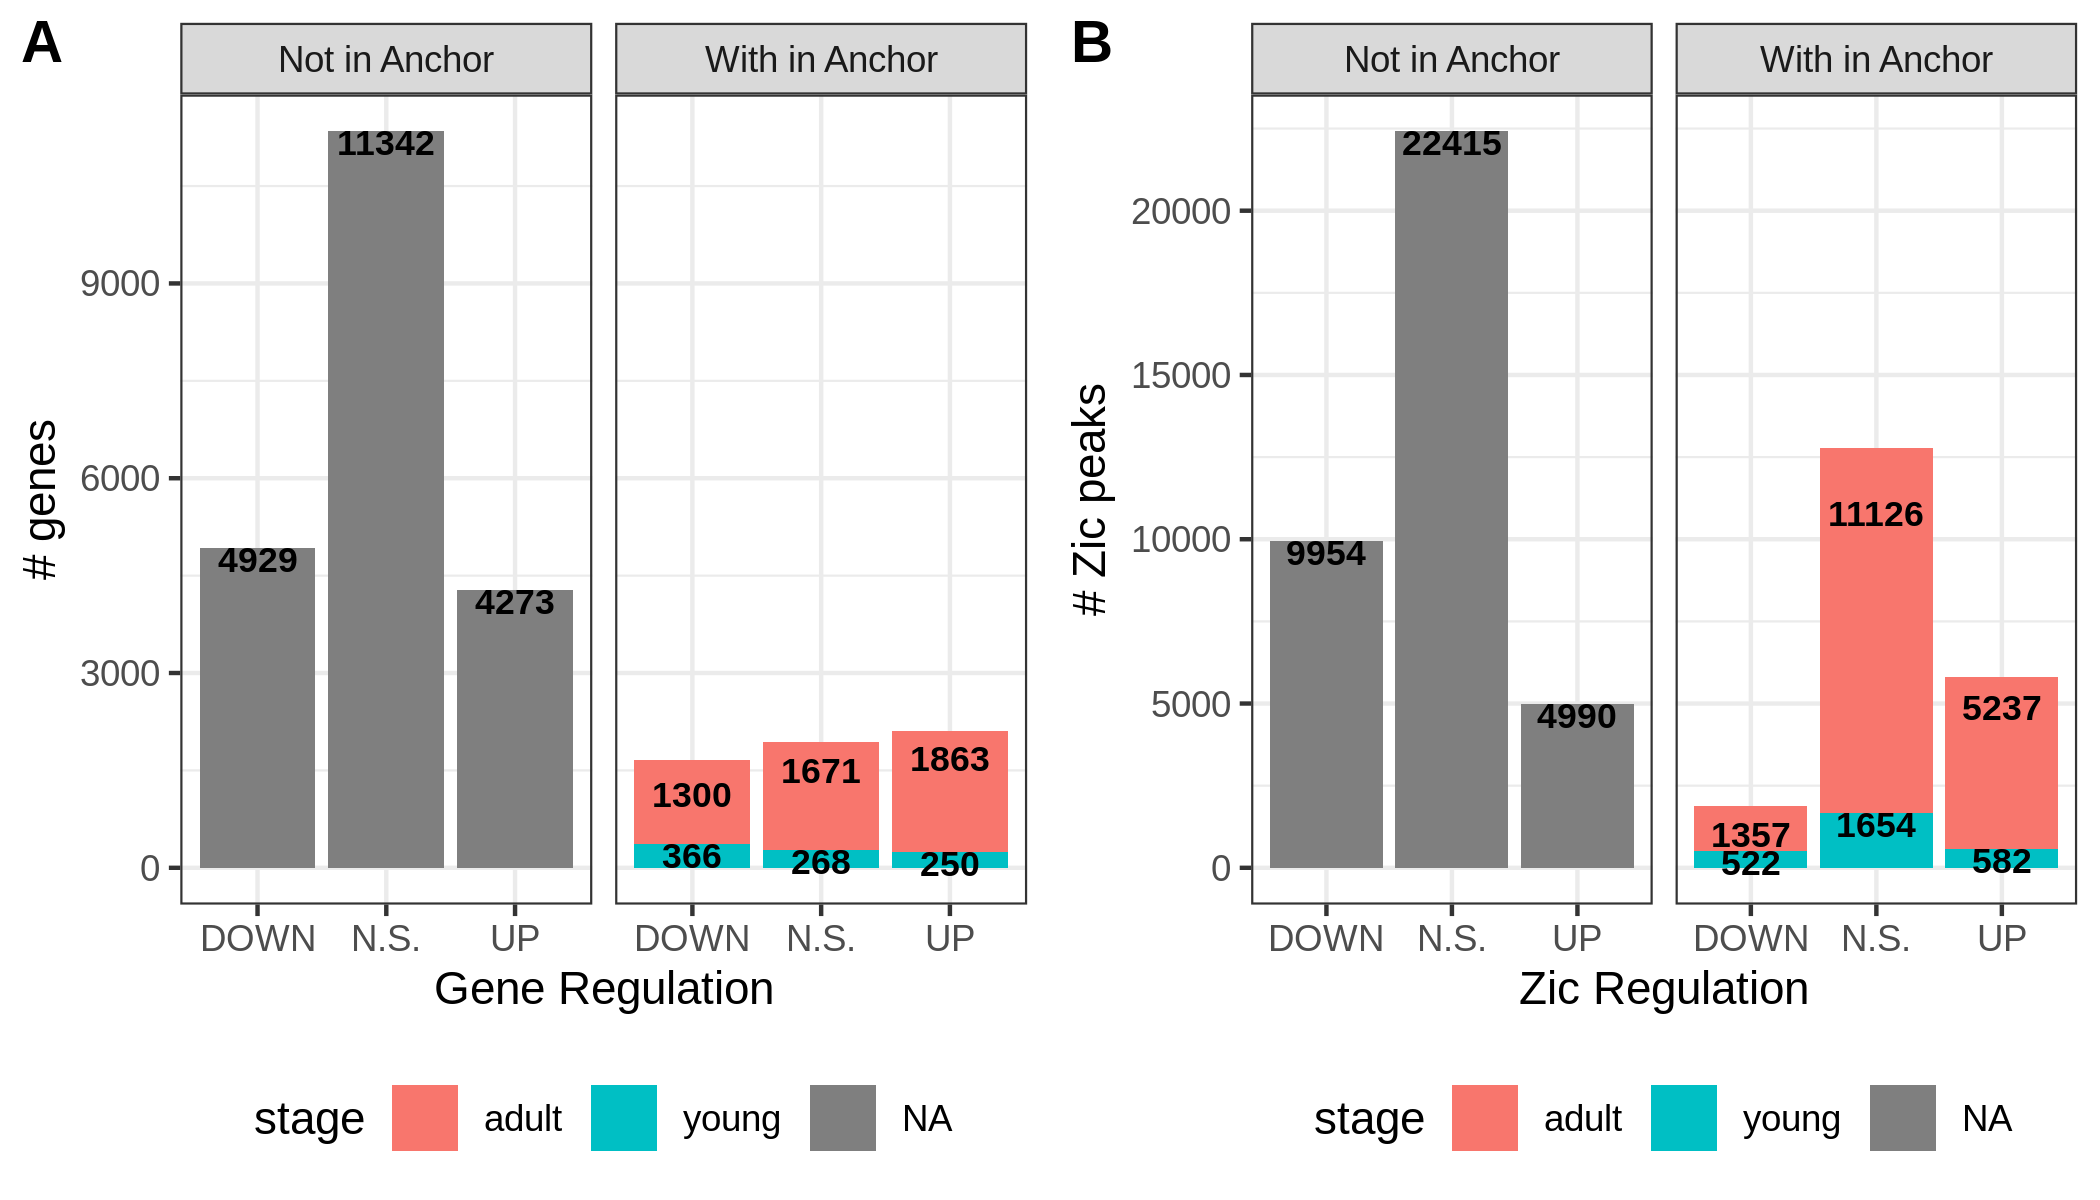
\includegraphics[width=.95\textwidth]{../figures/supp_figure2.png}
\caption{In-vivo ChIP overlap enrichment in orange (\textt{BART}) and motif enrichment in black (\texttt{HOMER}) of Zic ChIP peaks. A) Venn Diagram showing the overlap of the TFs within the Bart (orange) and Homer (black) databases. Significant TF motif (black) and in-vivo ChIP (orange) enrichment statistics where *Denotes predicted TFs that are common between the ChIP overlap enrichment and motif enrichment and TFs in blue indicates TFs that are in databases used by \texttt{Homer} and \texttt{BART} for all B) early and C) late Zic Zic peaks. Heatmap of RRHO p-values comparing the D) Motif and E) In-vivo ChIP enrichment of TFs in early and late Zic peaks}
\label{fig:HomerBart}
\end{figure*}

%\begin{figure*}[ht]
%\centering
%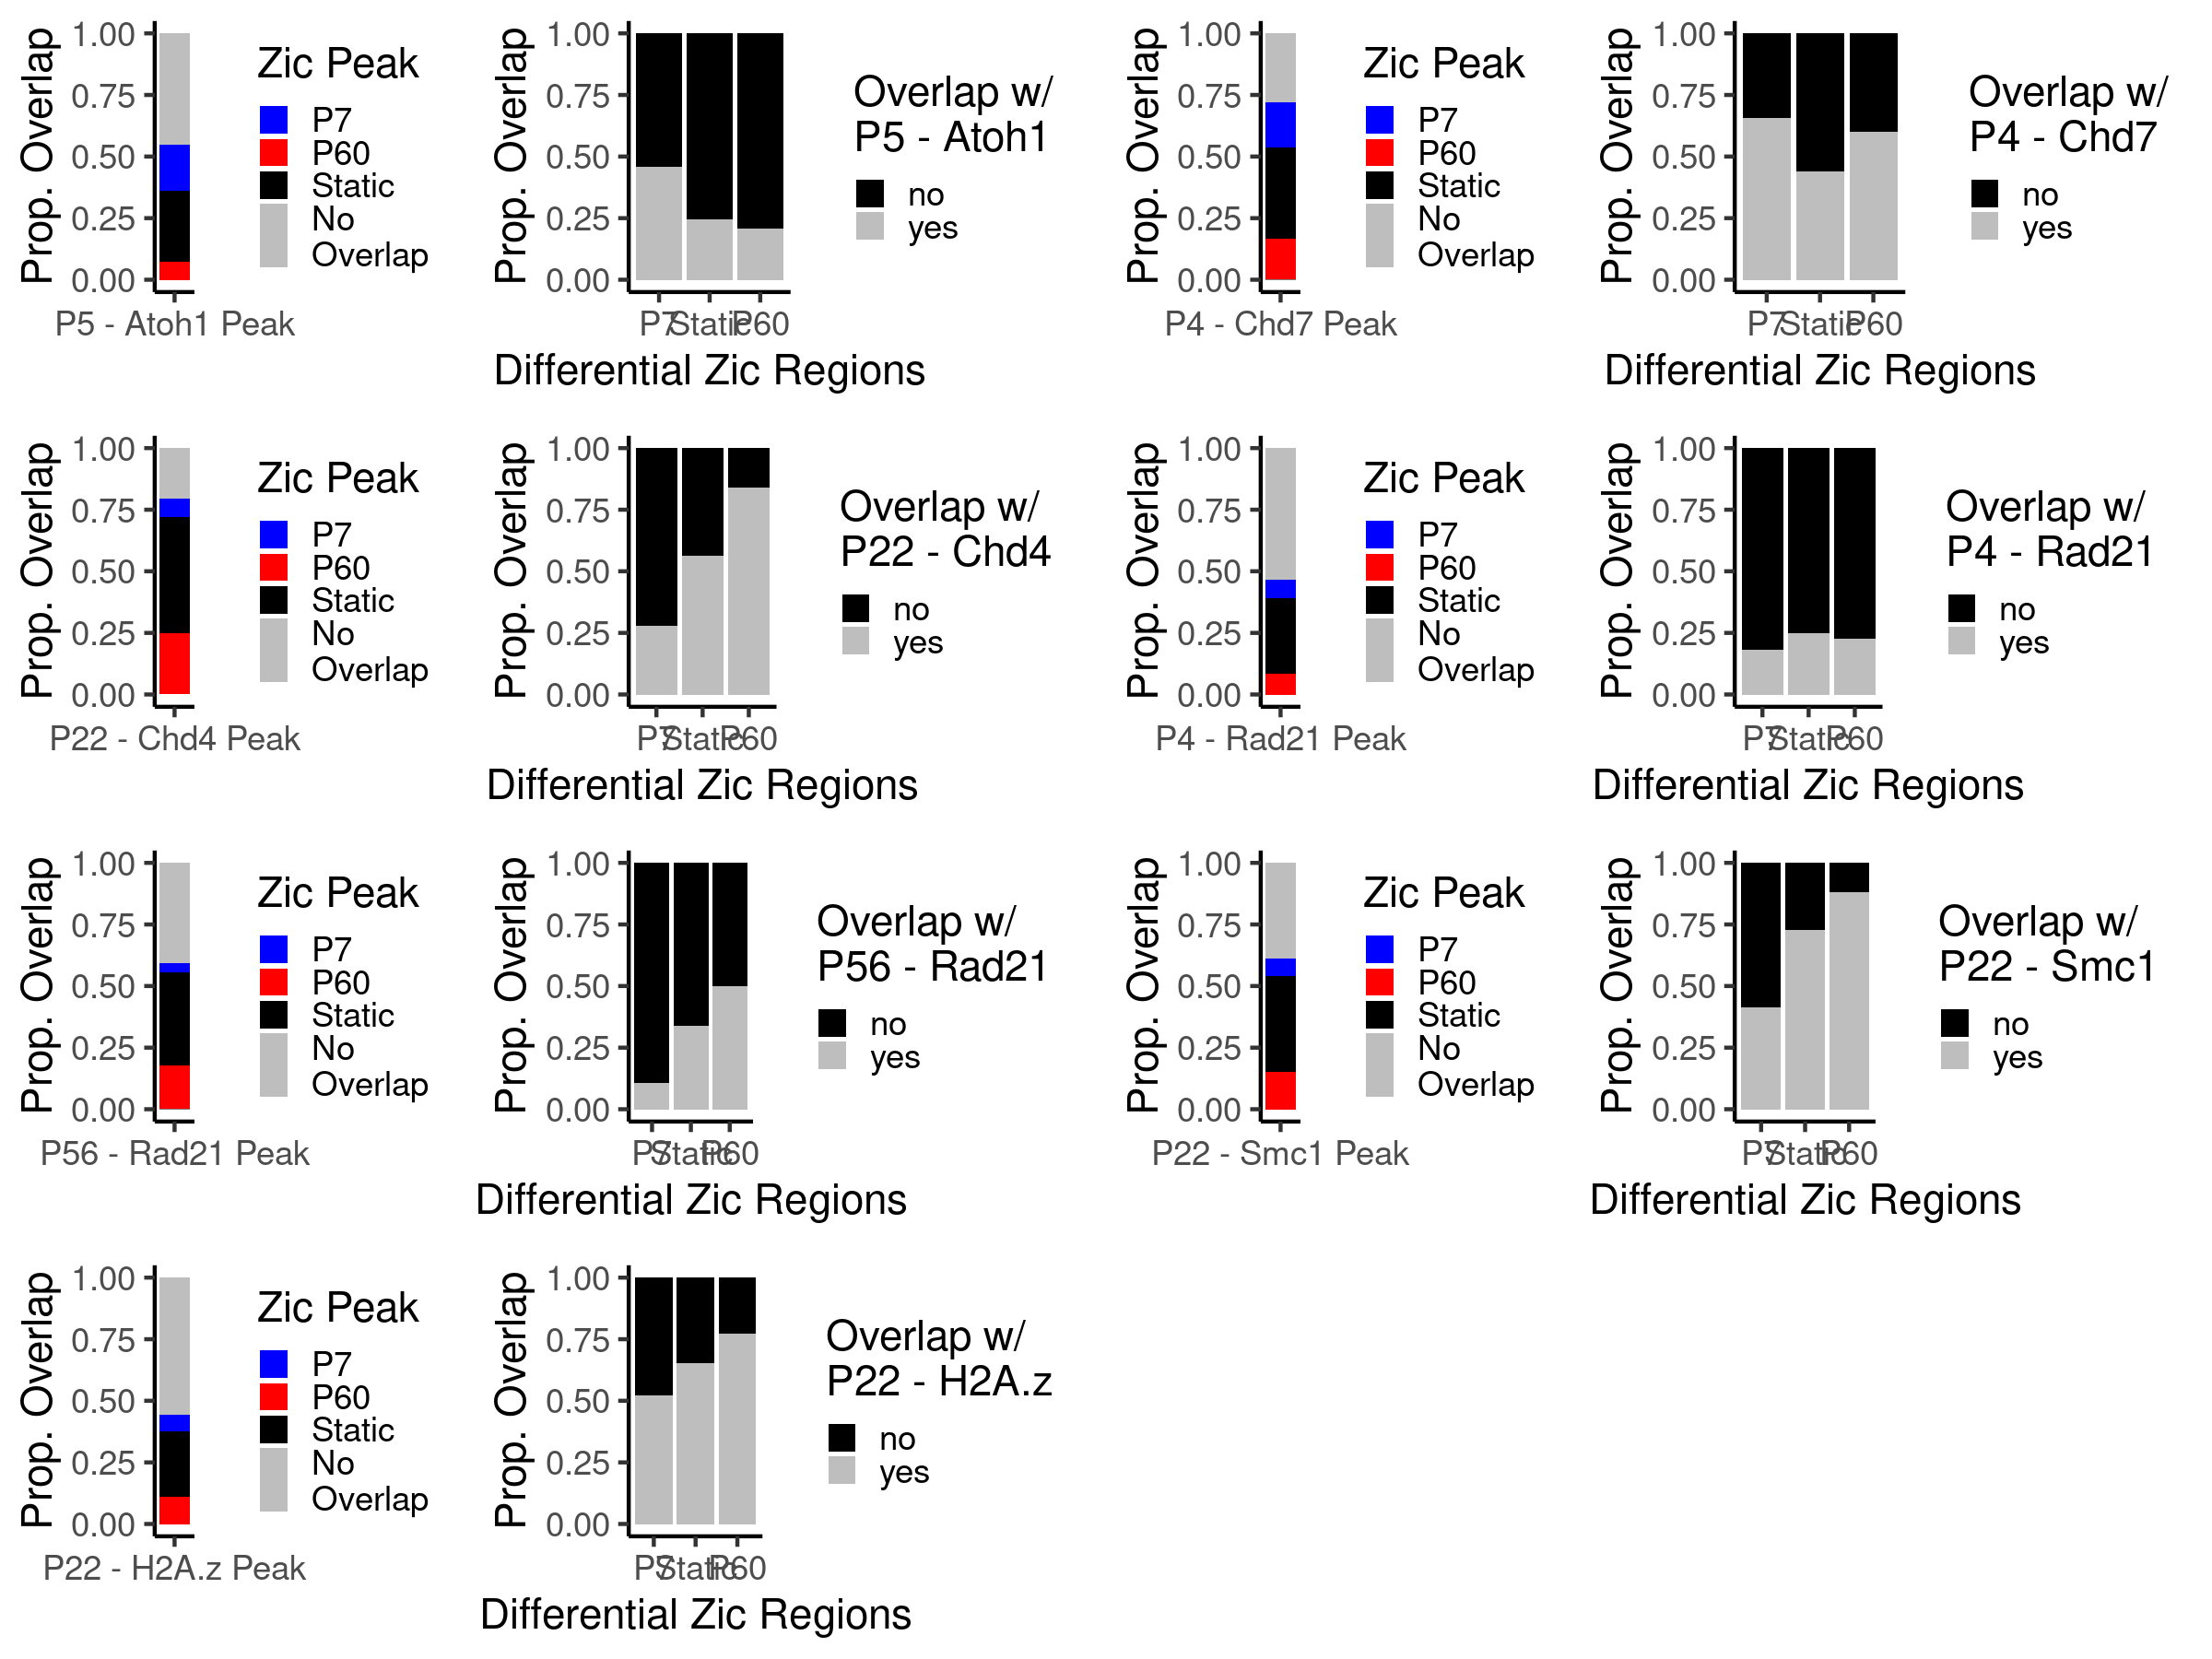
\includegraphics[width=.95\textwidth]{../figures/supp_figure_chip_overlap.png }
%\caption{Overlap Zic1/2 ChIP-seq and other ChIP-seq data in the developing cerebellum. The proportion of of ChiP peaks that are co-occupied by Zic peaks colored by the enrichment of the Zic peak (red - enriched at P60, blue - enriched at P7, black - static, and grey - no Zic peak) (Left) and the proportion of overlap (grey) or nonoverlap(black) of ChIP data sets that overlap Zic peaks separated by P7 enriched, static, and P60 enriched peaks (Right) for Atoh1 at P5 \cite{Klisch2011InDevelopment}, Chd4 at P22\cite{Yang2016ChromatinCoding}, Rad21 at P4 \cite{} and  P56 \cite{Reddy2021CHARGECerebellum}, H2A.z and P22 \cite{Yang2016ChromatinCoding}, Chd7 at P4 \cite{Reddy2021CHARGECerebellum}, Smc1 at P22 \cite{Goodman2020TheBrain}.  }
%\label{fig:chip_overlap}
%\end{figure*}


\begin{figure*}[ht]
\centering
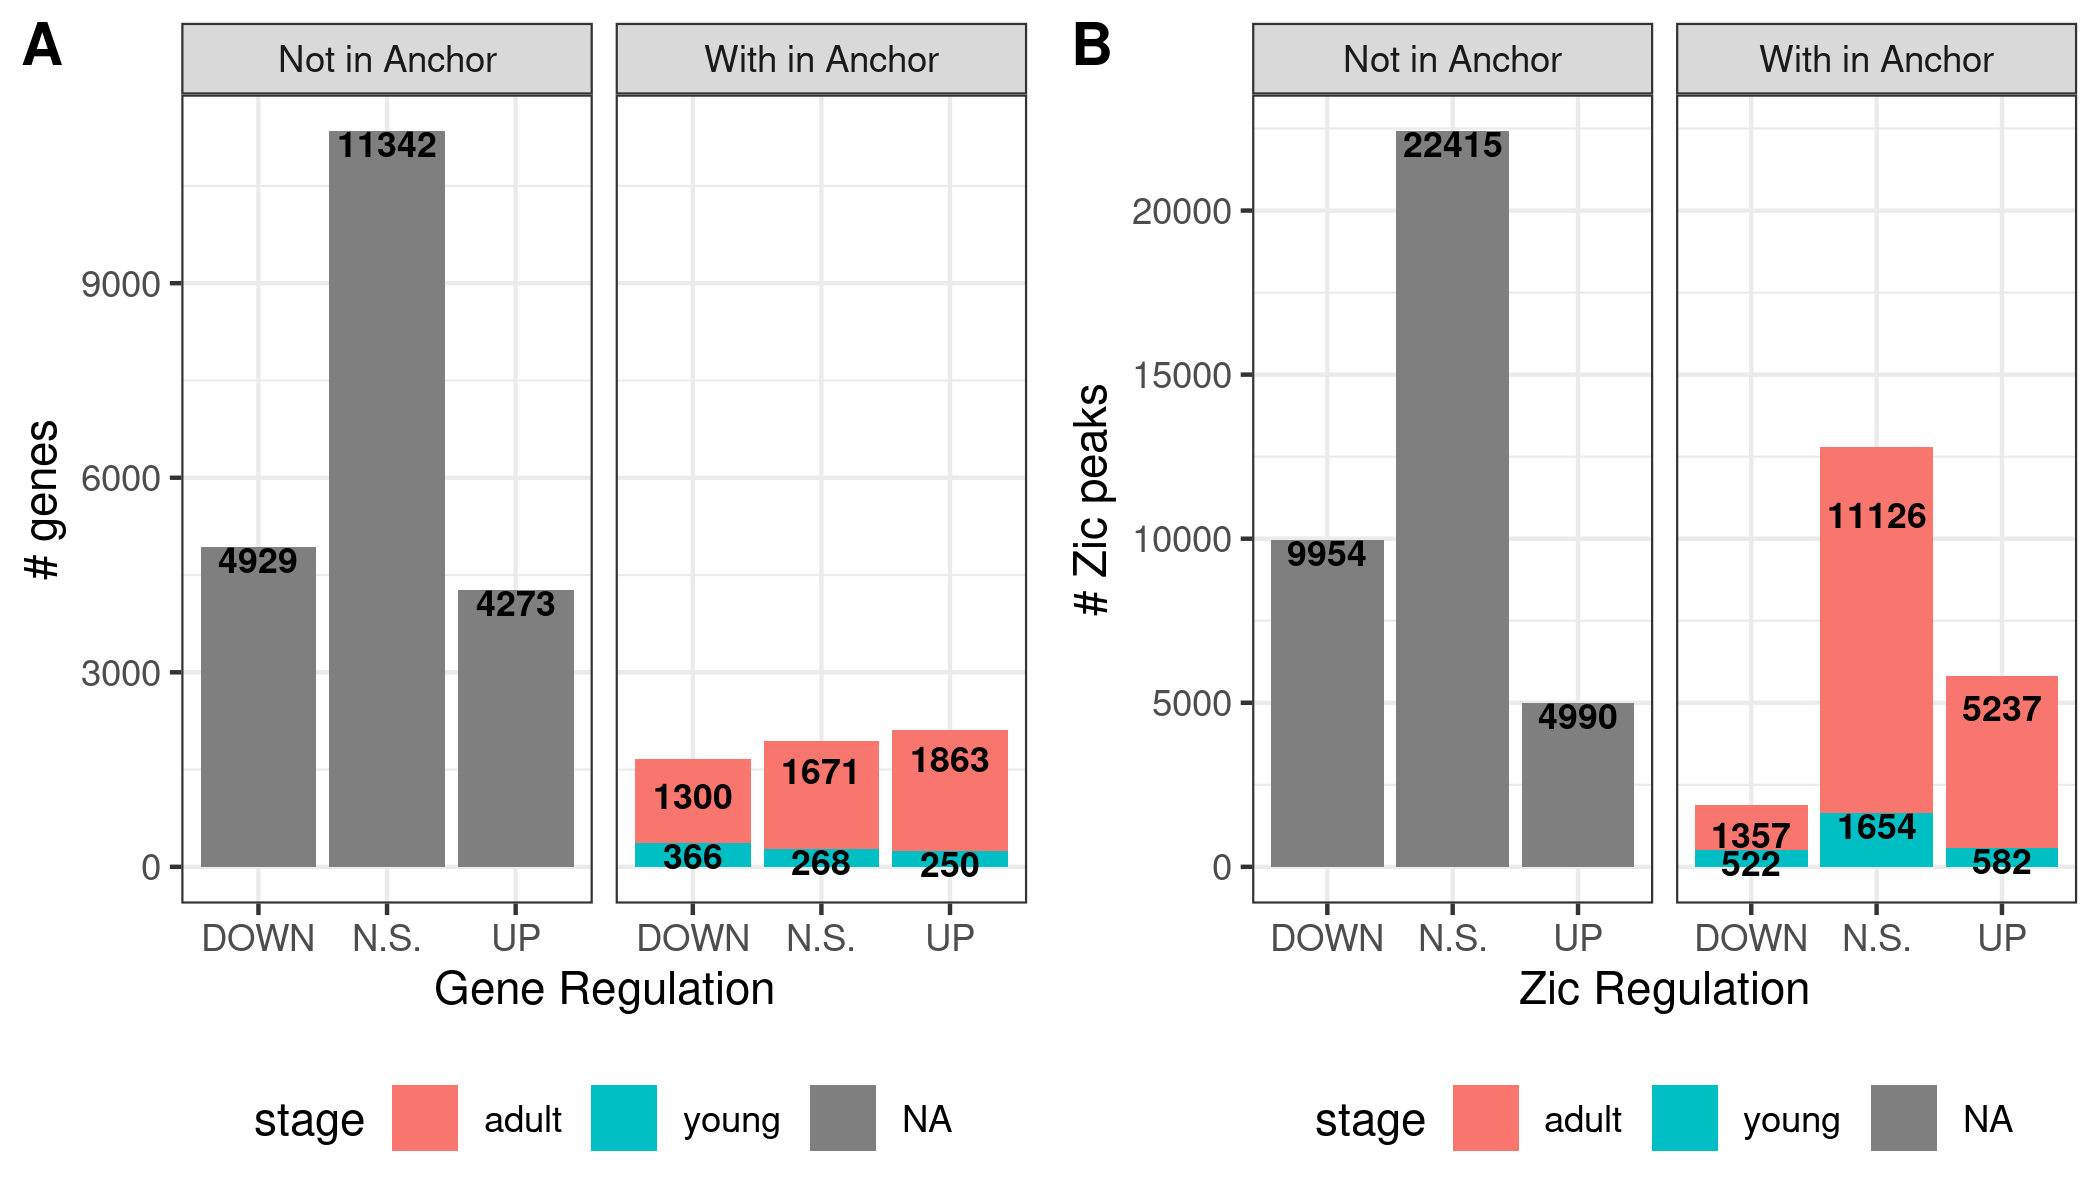
\includegraphics[width=.90\linewidth]{../figures/supp_figure_anchor.png}
\caption{ Identification of Zic peaks that overlap Hi-C anchors to facilitate enhancer-target gene identification. Number of Zic ChIP peaks that overlap P4 (young) Hi-C anchors from the Goodman et al. 2020 \cite{Goodman2020TheBrain} amd P56 (adult) PLAC-seq anchors from the Yamada et al. 2019 study \cite{Yamada2019SensoryLearning} sorted by A) the change in gene expression over time of the target gene and B) the change in Zic binding over time of the Zic peaks that overlap the anchors.}
\label{fig:MappingStats}
\end{figure*}


\begin{figure*}[ht]
\centering
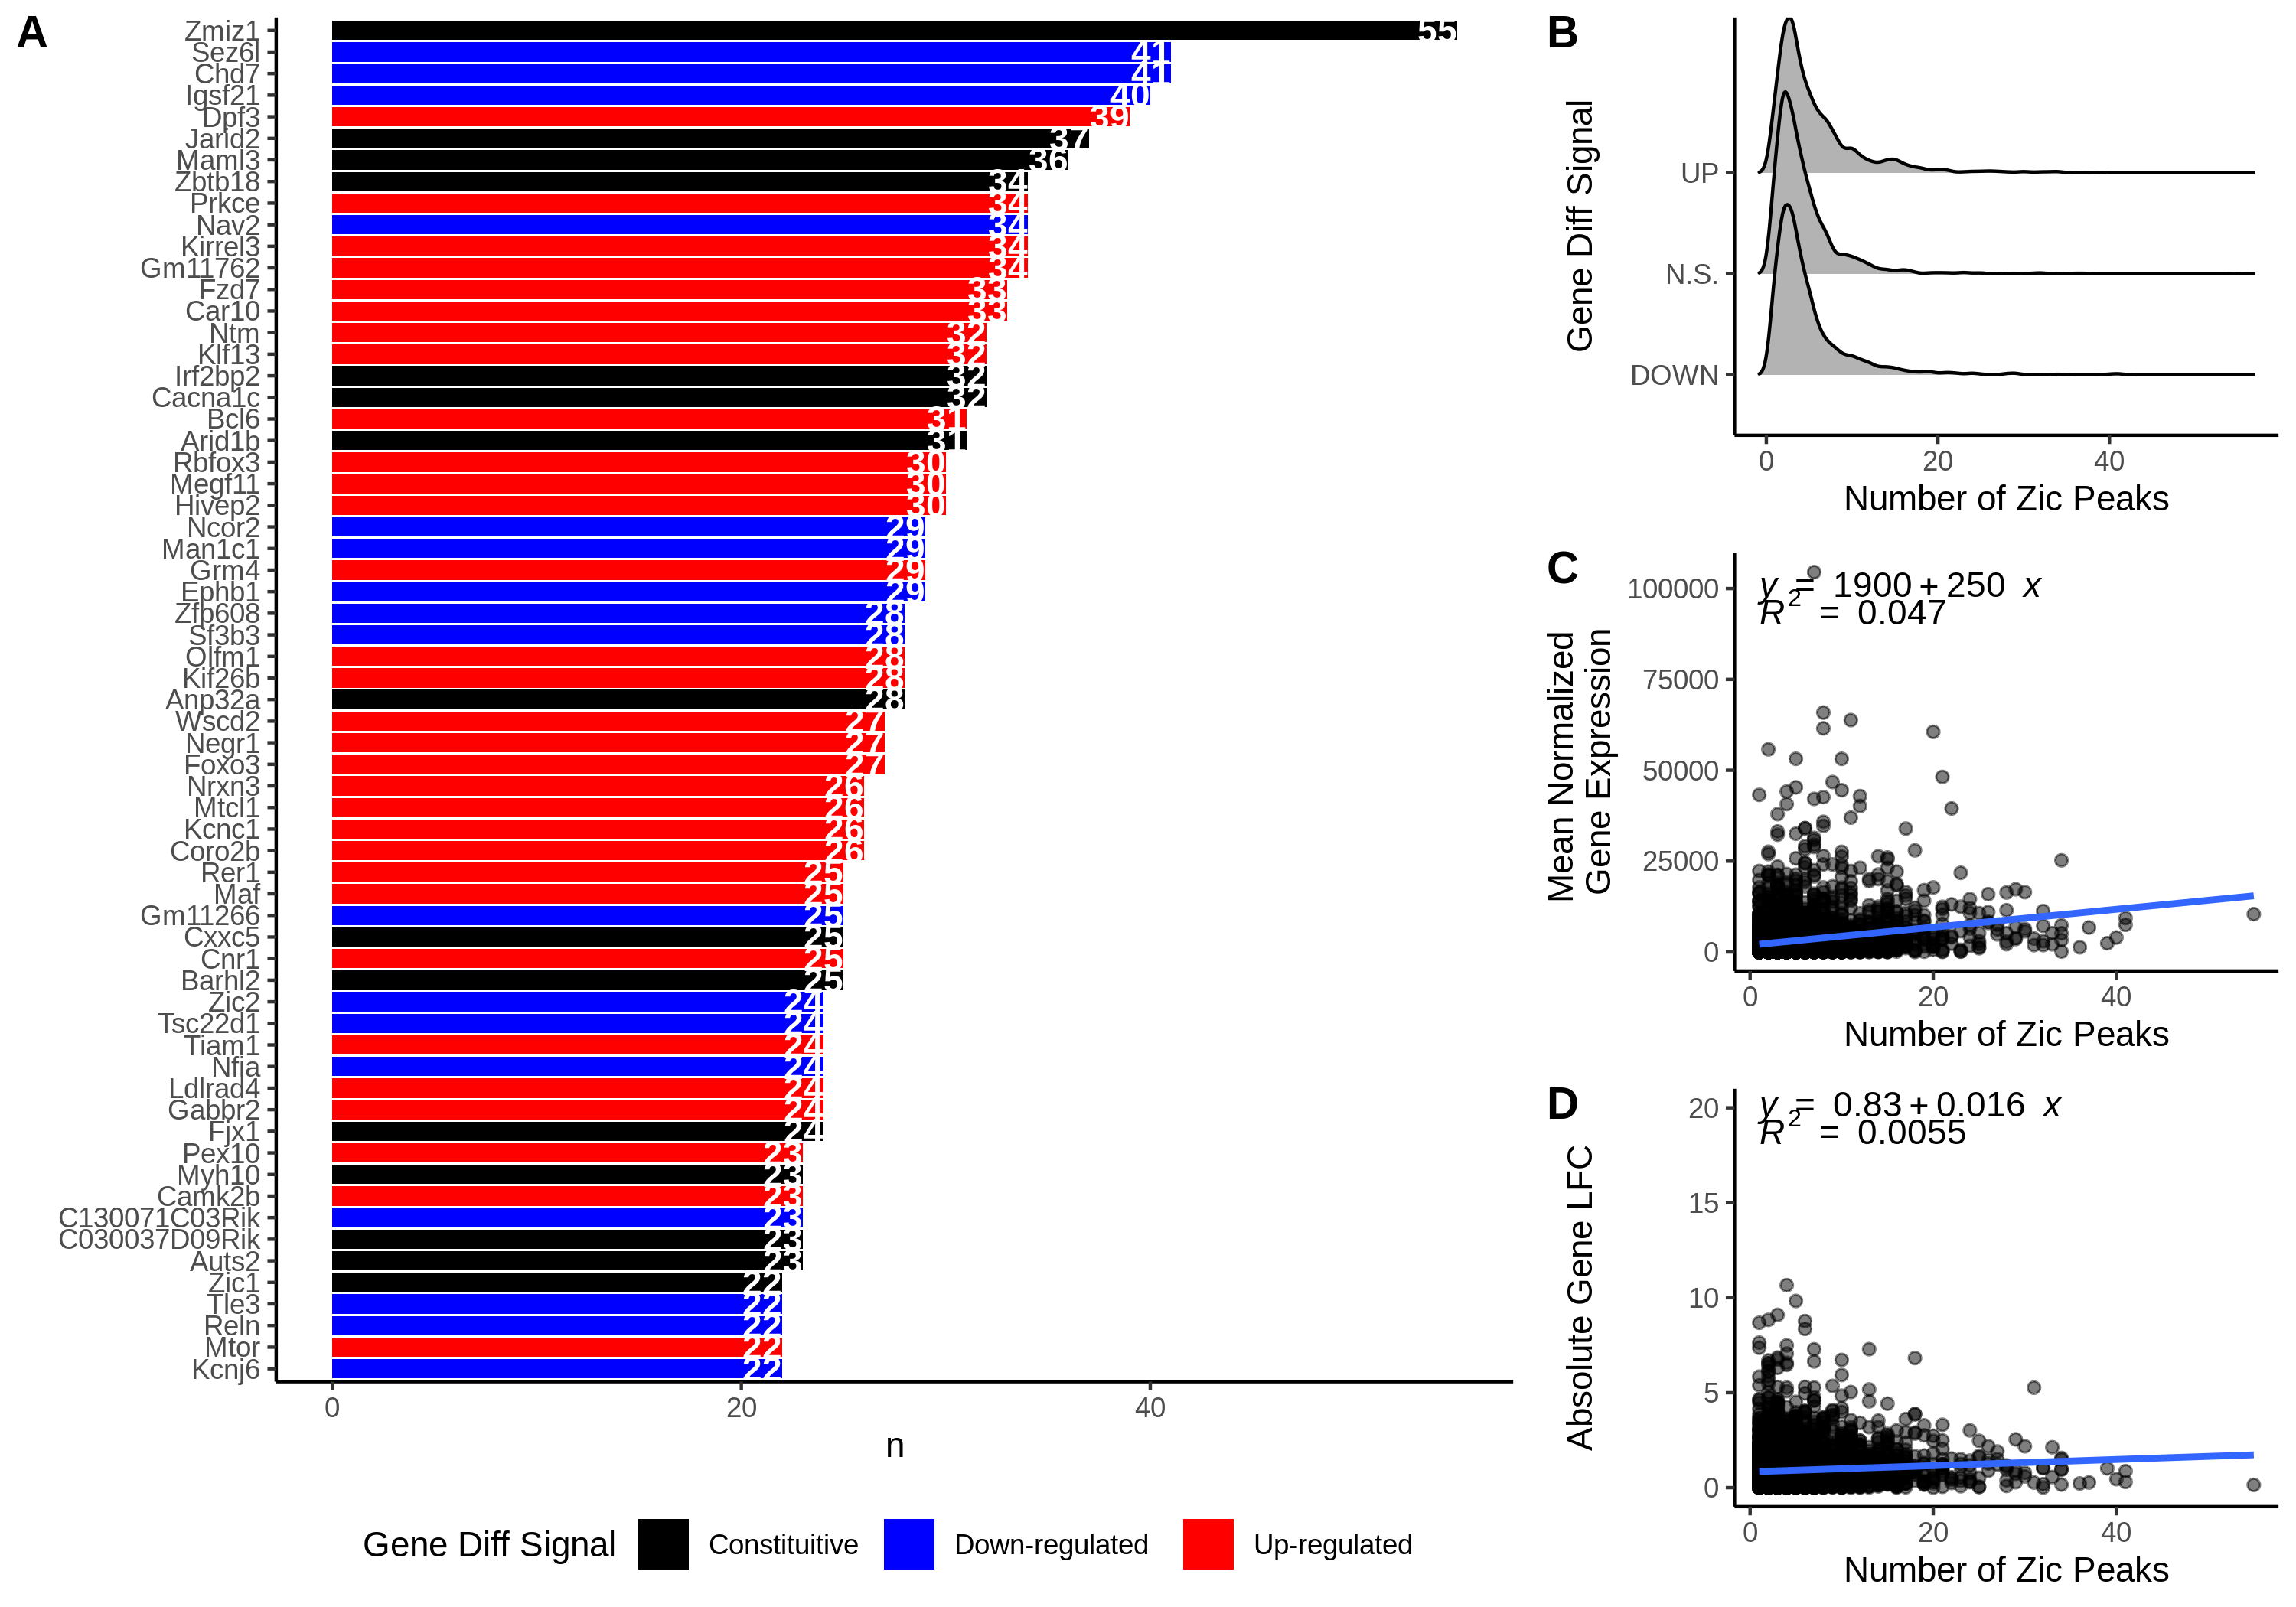
\includegraphics[width=.90\linewidth]{../figures/supp_figure3.png}
\caption{ The number of Zic peaks that map to a target gene does not correlate with the direction of gene regulation over developmental time A) Count of Zic peaks mapped to gene where the color indicates whether the gene is up-regulated (red), down-regulated (blue) or constitutively expressed (black). B) Distribution densities of number of Zic peaks by gene regulation.  Scatter-plots of C) Mean expression and D) absolute log fold change of genes versus the number of Zic peaks. }
\label{fig:npeakstoGenes}
\end{figure*}


\begin{figure*}[ht]
\centering
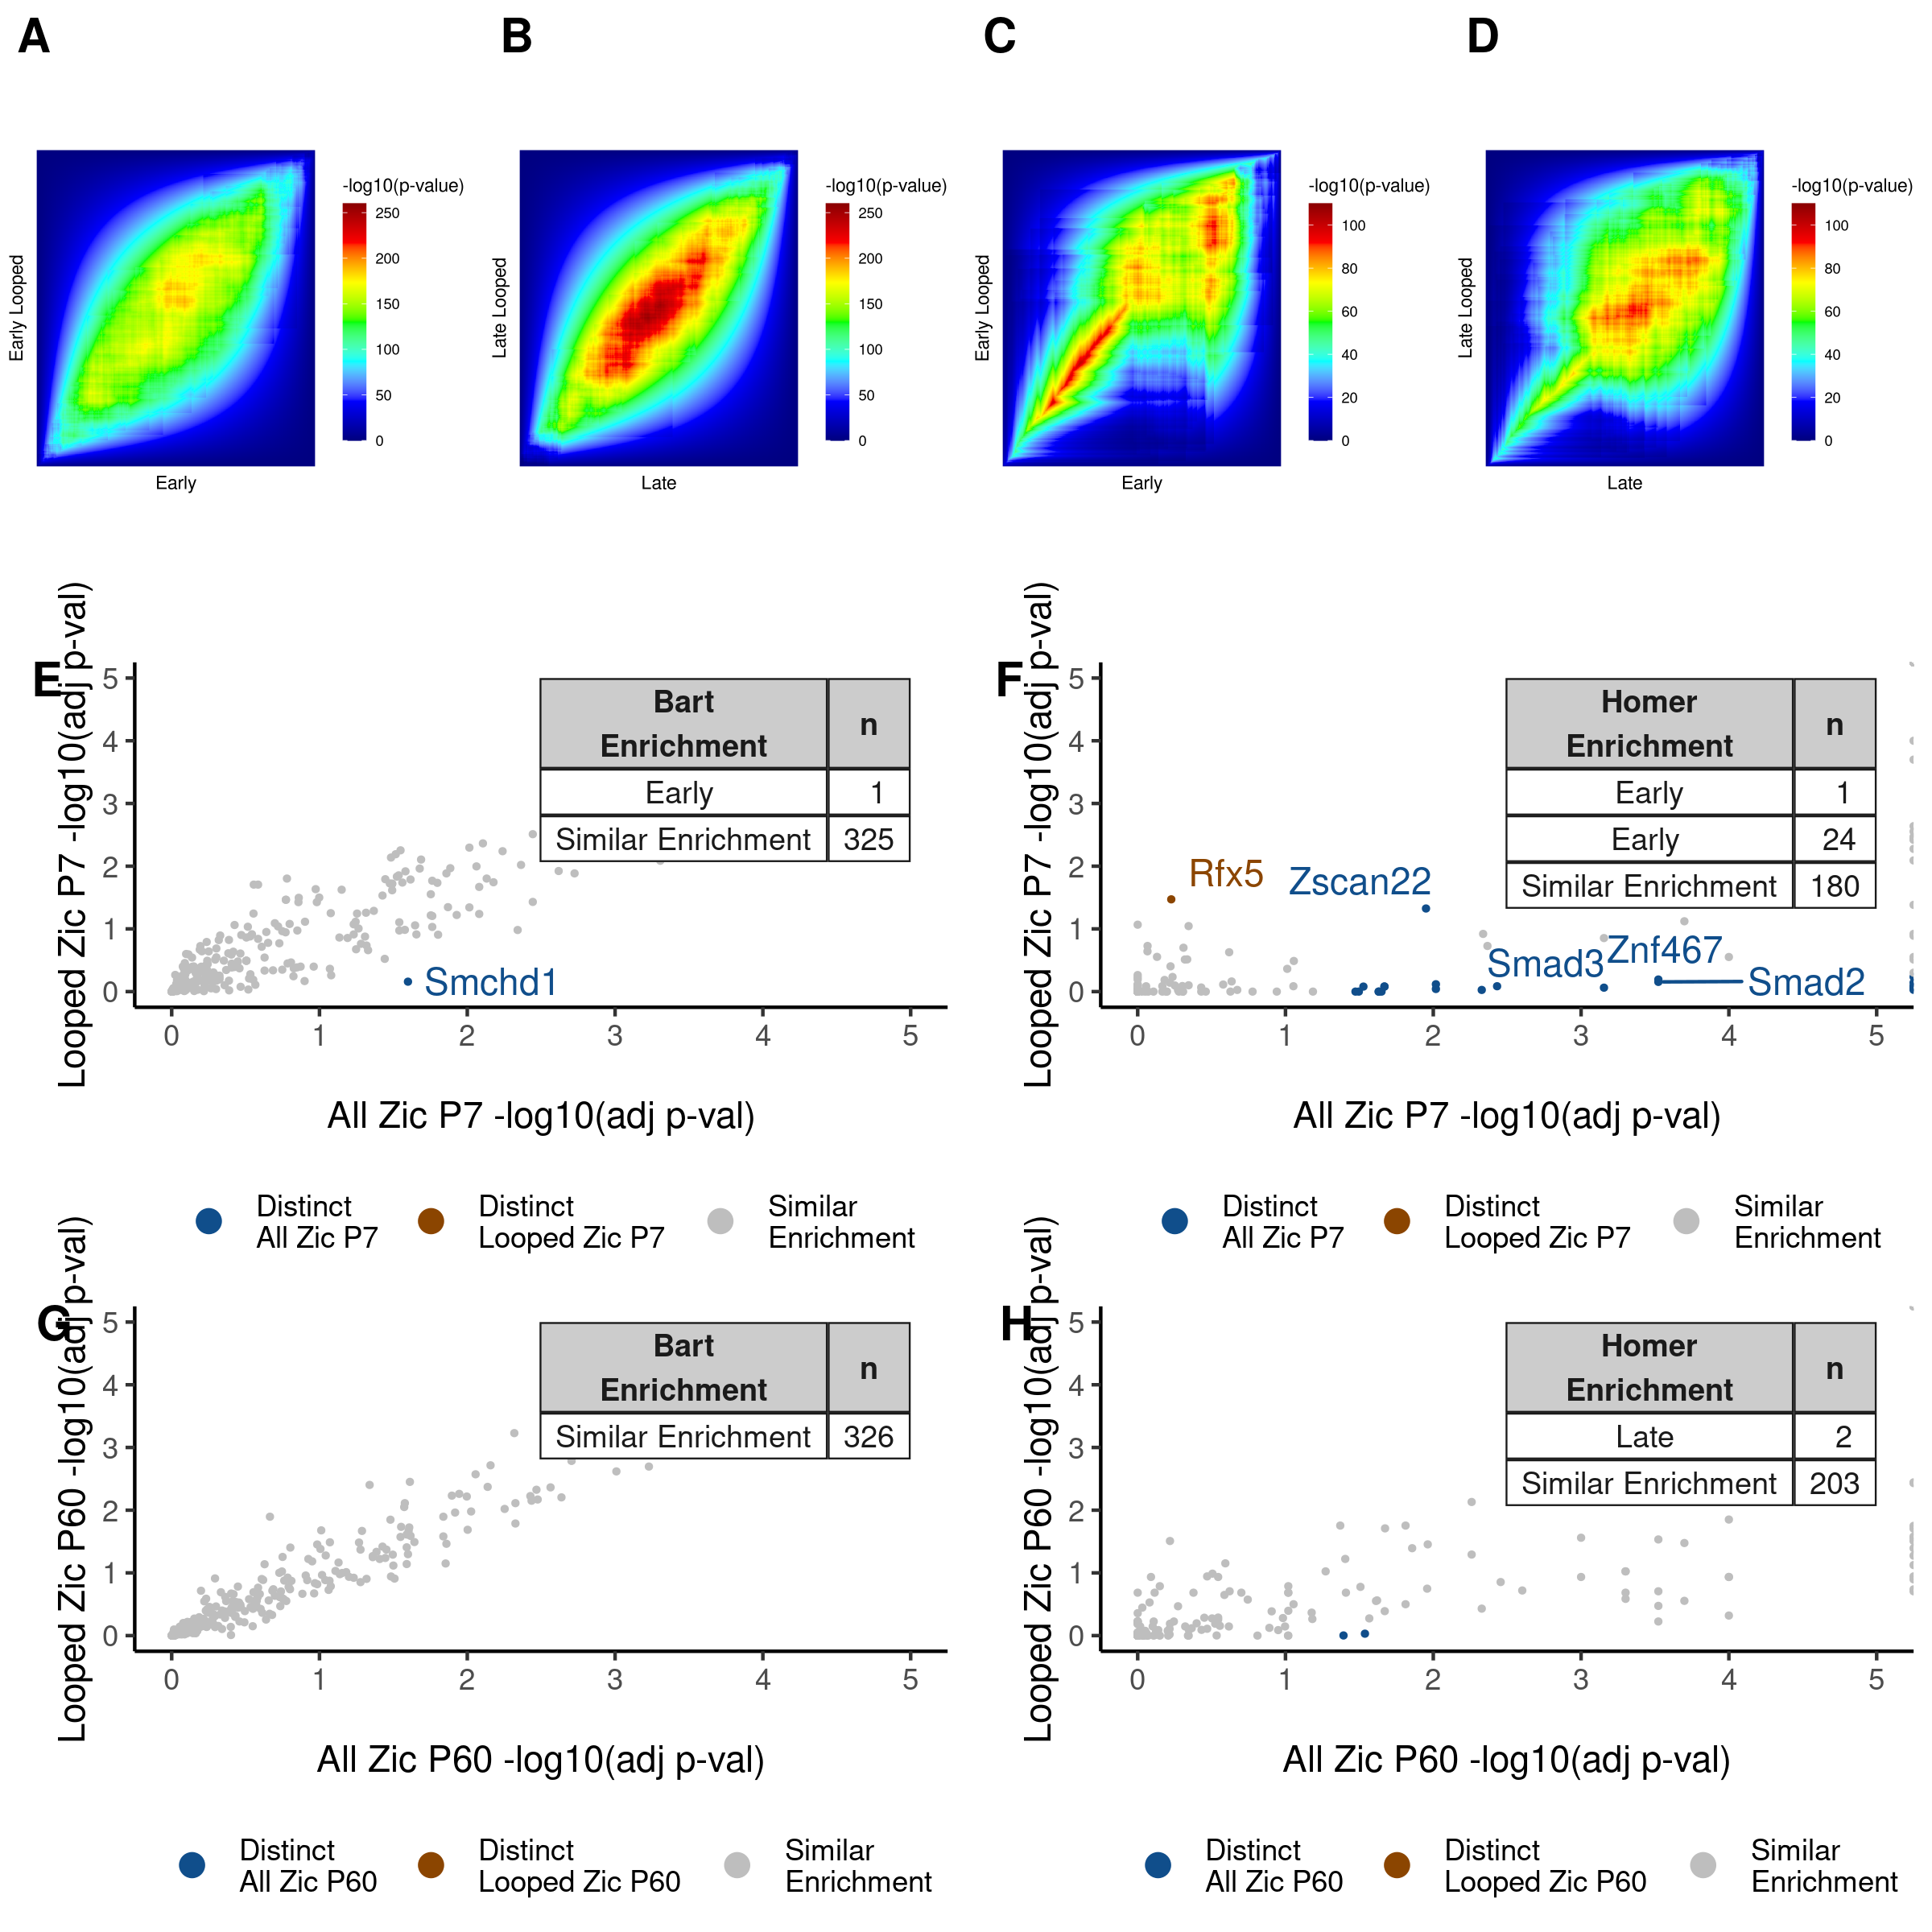
\includegraphics[width=.95\textwidth]{../figures/supp_figure_rrho_allvlooped.png}
\caption{Distinct TFs between the all Zic1/2 ChIP sites and the ones within anchors. Heatmap of RRHO p-values comparing the Motif enrichment between A) all early and lopped early Zic peaks, B) All late and looped late Zic peaks. As well as comparing the in-vivo ChIP enrichment of TFs between C) all early and lopped early Zic peaks D) All late and looped late Zic peaks. Scatter-plot of the enrichment p-values for each TF in each category colored by whether a TF was distinctly enriched as calculated by the RRHO analysis between all early Zic peaks and early Zic peaks within chromatin loop anchors  all late peaks and late peaks within chromatin loop anchors using the output from E,G)\texttt{BART} and F,H )\texttt{Homer}.  }
\label{fig:loopved_all}
\end{figure*}

\begin{figure*}[!ht]
\centering
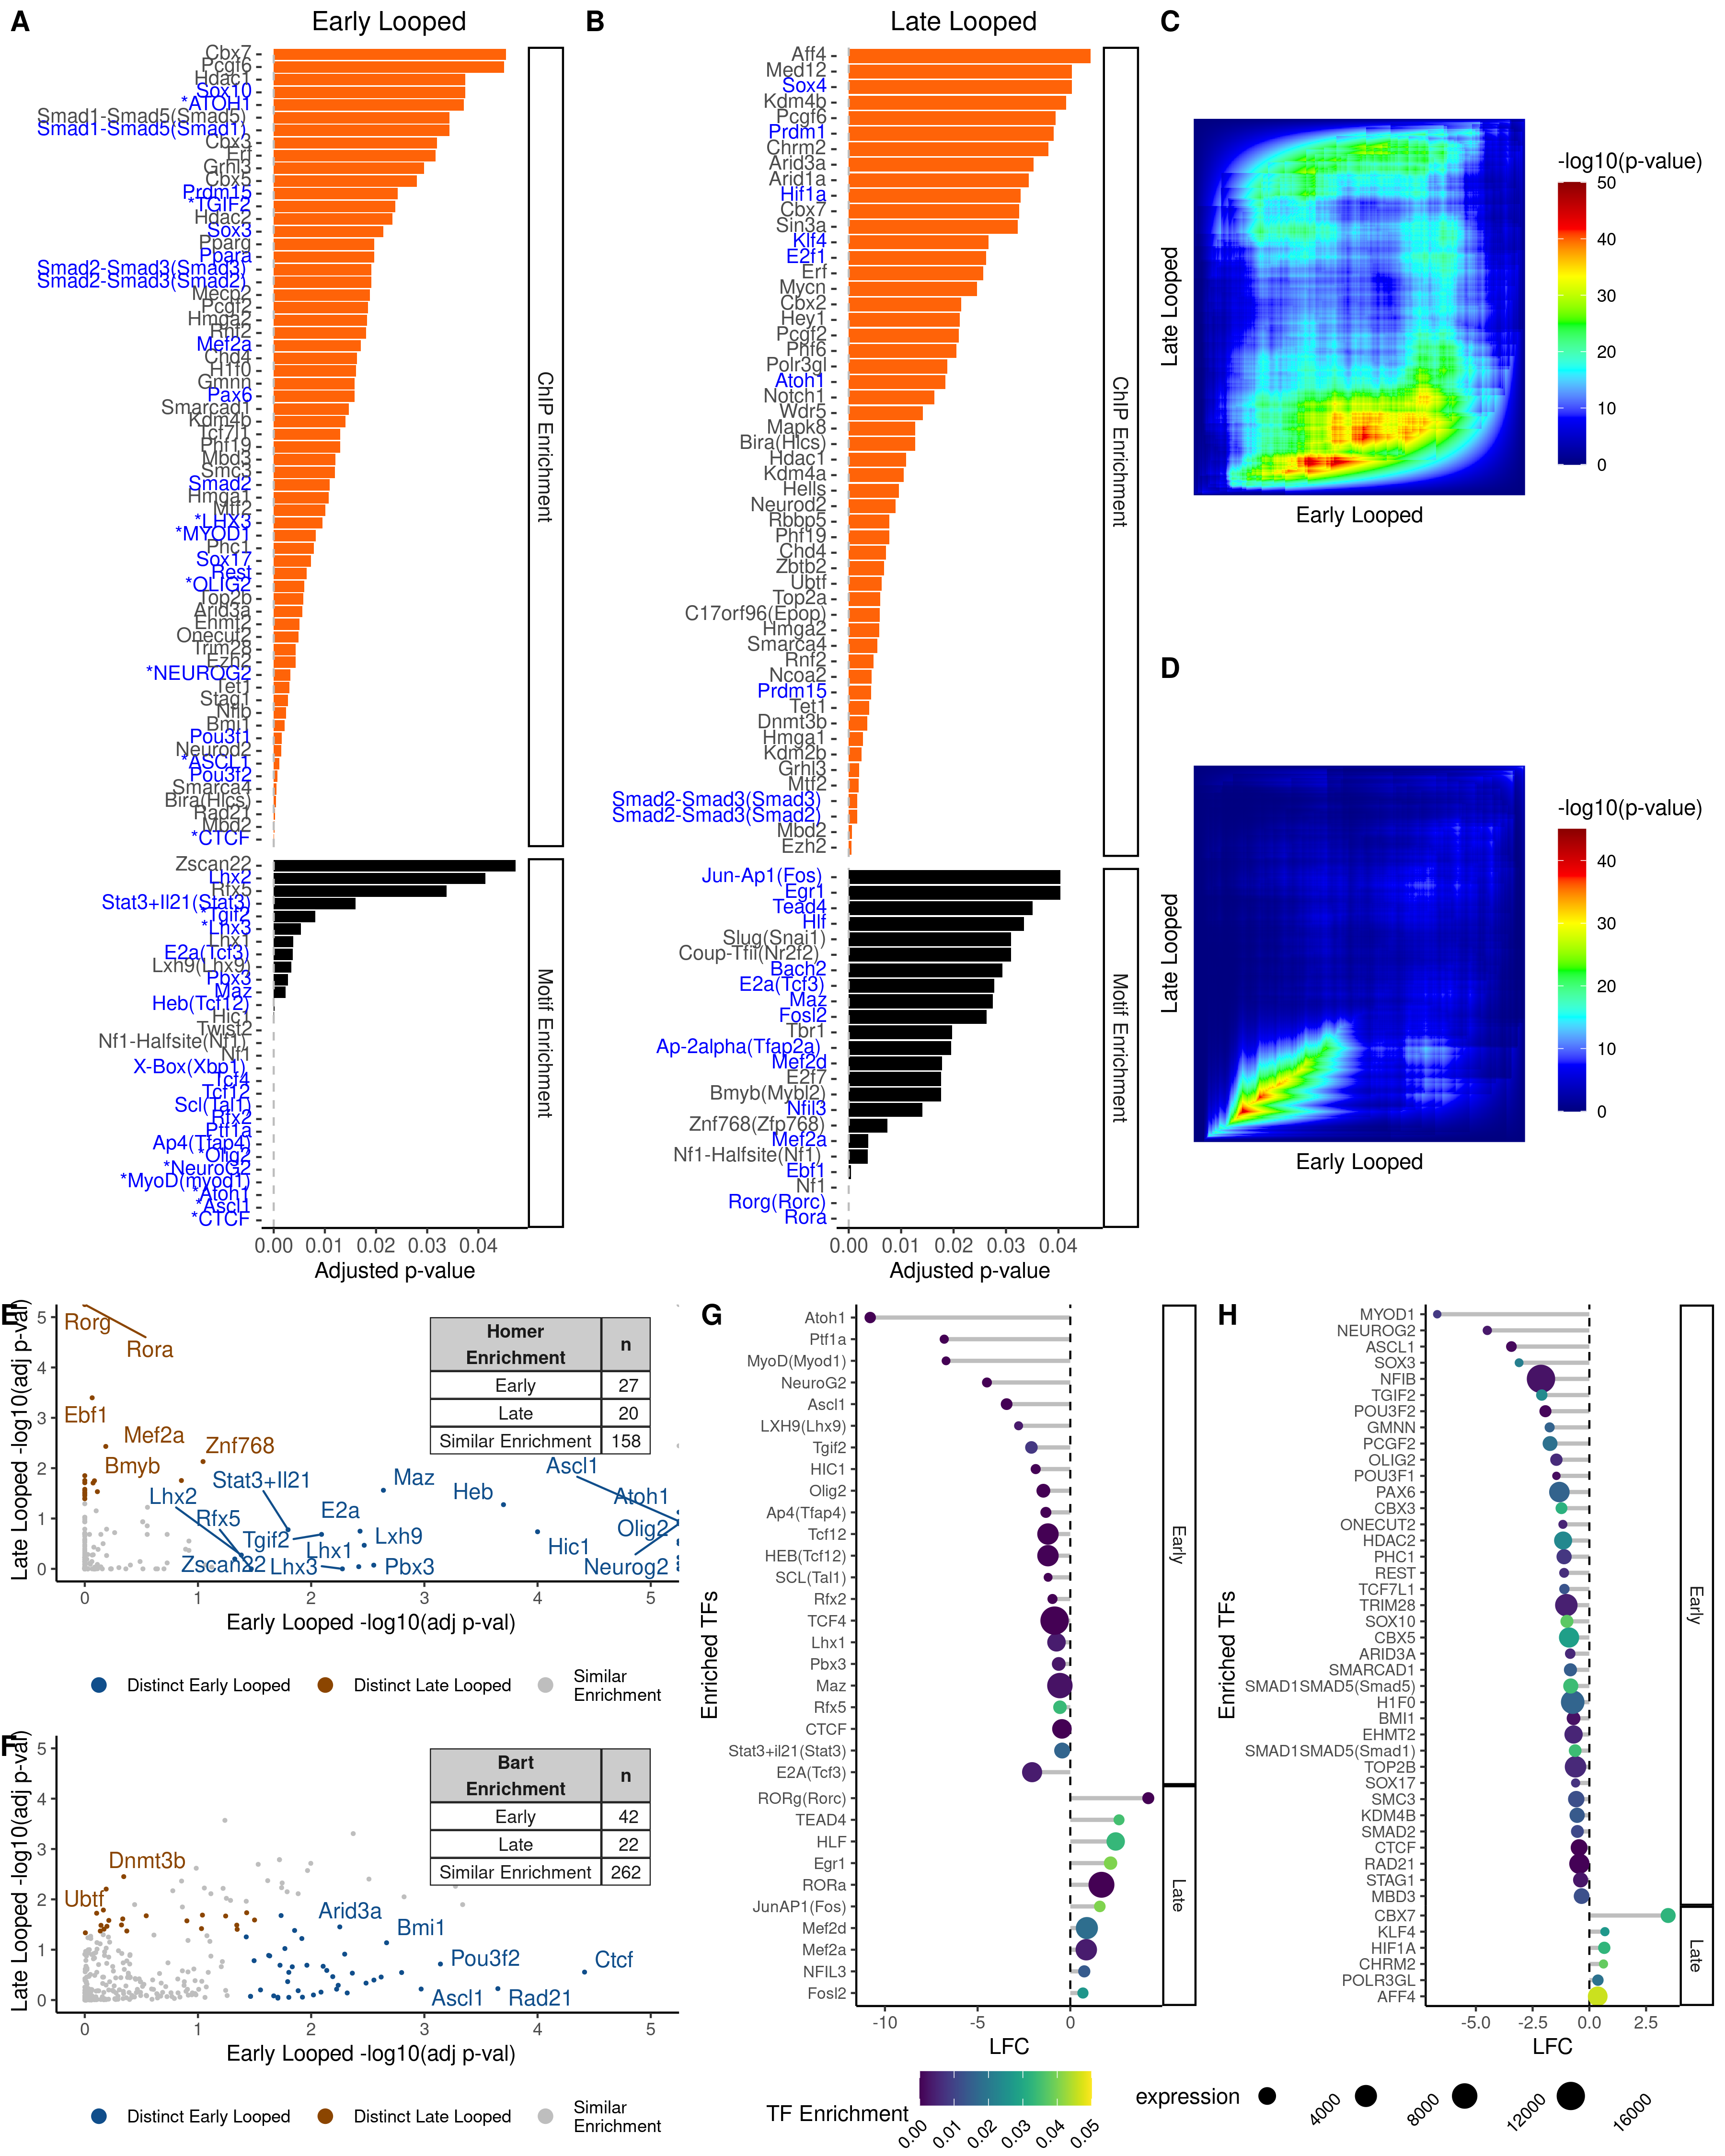
\includegraphics[width=.95\textwidth]{../figures/figure2_loop.png}
\caption{ Distinct TFs are enriched between early and late Zic binding within chromatin loop anchors. Significant TF motif (black) and in-vivo ChIP (orange) enrichment statistics where *Denotes predicted TFs that are common between the ChIP overlap enrichment and motif enrichment and TFs in blue indicates TFs that are in databases used by \texttt{Homer} and \texttt{BART} for looped A) early and B) late Zic Zic peaks.  Heatmap of RRHO p-values comparing the C) Motif and D) In-vivo ChIP enrichment of TFs in early and late Zic peaks. Distinctly enriched E) motifs and F) ChIP profiles between looped  early and late Zic sites. These TFs G) motifs and H) ChIP profiles in looped early and late Zic sites were filtered for transcriptional enrichment at the respective time-points. The size of each point is the average expression of the mapped gene at the respective time point.}
\label{fig:DistinctTFs_looped}
\end{figure*}




\begin{figure*}[!ht]
\centering
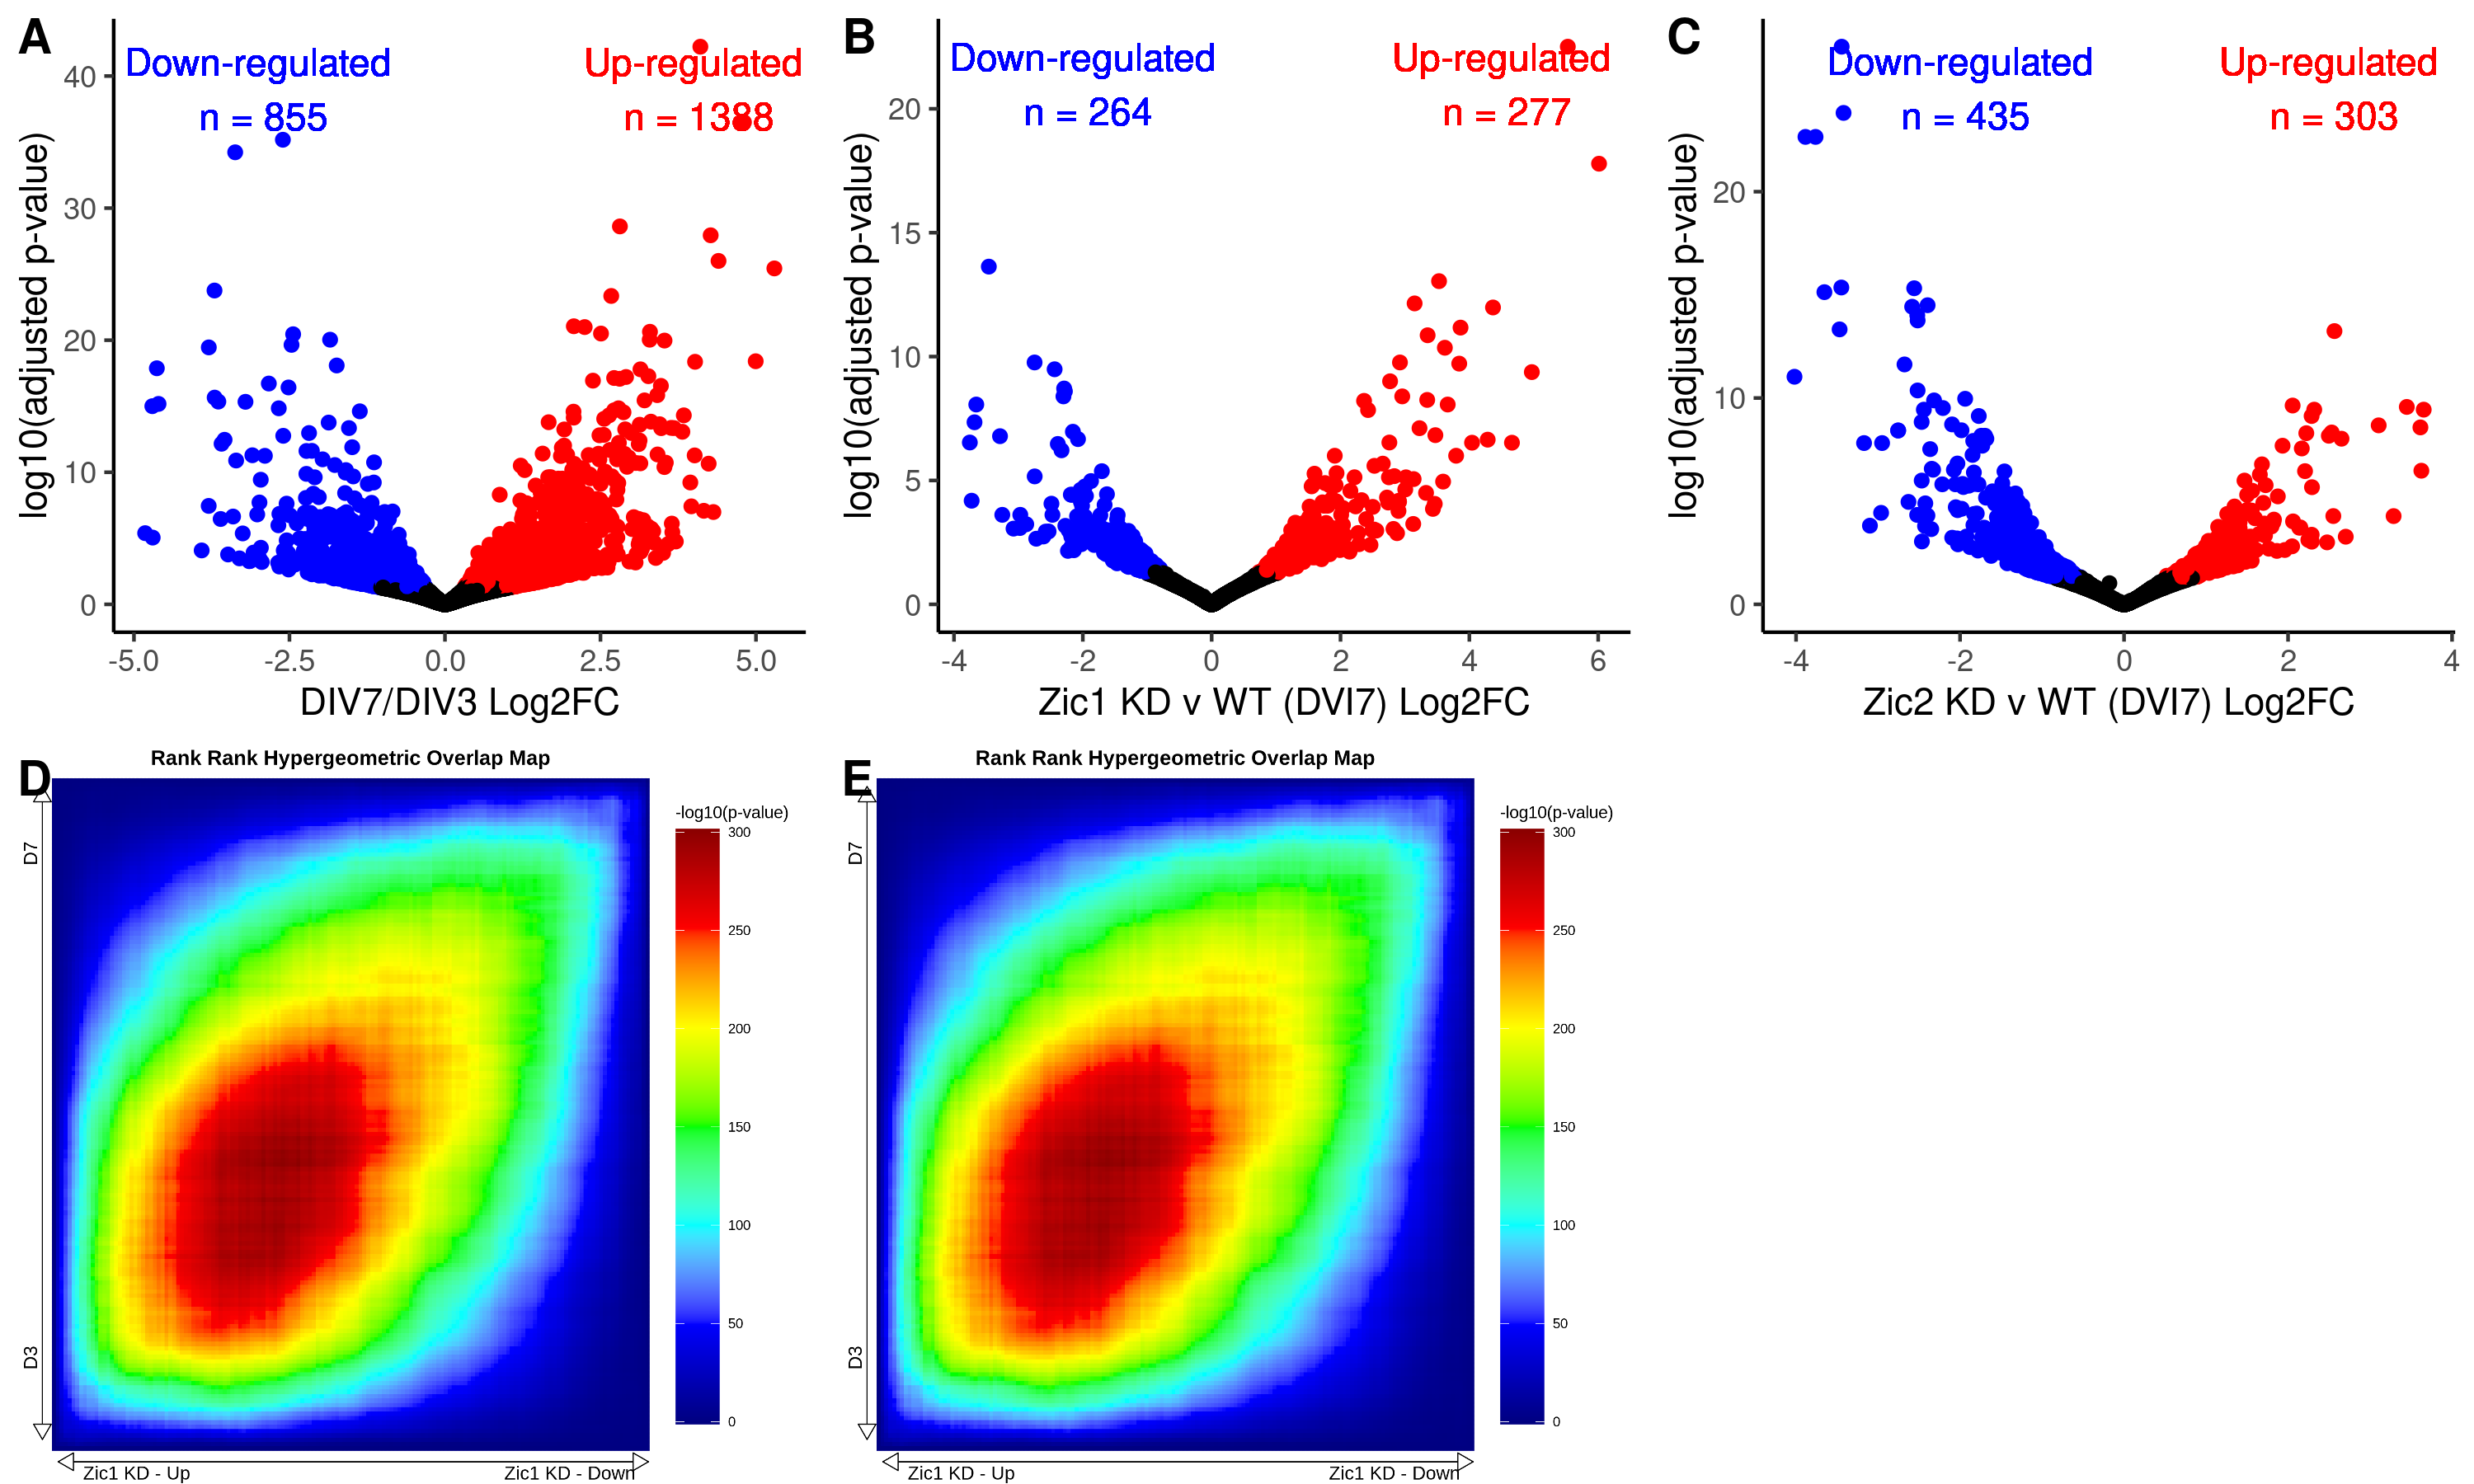
\includegraphics[width=.95\textwidth]{../figures/supp_figure_vitro.png}
\caption{ [need title]. Volcano plots showing the differential genes between A) DIV7 v DIV3, B) Zic1 KD v WT at DIV7 C) Zic2 KD v WT at DIV7. Heatmap of RRHO p-values comparing genes changing throughout WT  development versus D) with Zic1 knocked down and E) with Zic2 knocked down }
\label{fig:vitro}
\end{figure*}



\end{document}